% **************************************************************************************************************
% A Classic Thesis Style
% An Homage to The Elements of Typographic Style
%
% Copyright (C) 2012 Andr\'e Miede http://www.miede.de
%
% If you like the style then I would appreciate a postcard. My address 
% can be found in the file ClassicThesis.pdf. A collection of the 
% postcards I received so far is available online at 
% http://postcards.miede.de
%
% License:
% This program is free software; you can redistribute it and/or modify
% it under the terms of the GNU General Public License as published by
% the Free Software Foundation; either version 2 of the License, or
% (at your option) any later version.
%
% This program is distributed in the hope that it will be useful,
% but WITHOUT ANY WARRANTY; without even the implied warranty of
% MERCHANTABILITY or FITNESS FOR A PARTICULAR PURPOSE.  See the
% GNU General Public License for more details.
%
% You should have received a copy of the GNU General Public License
% along with this program; see the file COPYING.  If not, write to
% the Free Software Foundation, Inc., 59 Temple Place - Suite 330,
% Boston, MA 02111-1307, USA.
%
% **************************************************************************************************************
% Note:
%    * You must not use "u etc. in strings/commands that will be spaced out (use \"u or real umlauts instead)
%    * New enumeration (small caps): \begin{aenumerate} \end{aenumerate}
%    * For margin notes: \marginpar or \graffito{}
%    * Do not use bold fonts in this style, it is designed around them
%    * Use tables as in the examples
%    * See classicthesis-preamble.sty for useful commands
% **************************************************************************************************************
% To Do:
%		 * [high] Check this out: http://www.golatex.de/koma-script-warnung-in-verbindung-mit-listings-package-t2058.html
%    * [medium] mathbb in section-titles/chapter-titles => disappears somehow in headlines!!!
% **************************************************************************************************************
\documentclass[ twoside,openright,titlepage,numbers=noenddot,headinclude,%1headlines,% letterpaper a4paper
                footinclude=true,cleardoublepage=empty,abstractoff, % <--- obsolete, remove (todo)
                BCOR=5mm,paper=a4,fontsize=11pt,%11pt,a4paper,%
                american,openany%
                ]{scrreprt}

%********************************************************************
% Note: Make all your adjustments in here
%*******************************************************
% ****************************************************************************************************
% classicthesis-config.tex 
% formerly known as loadpackages.sty, classicthesis-ldpkg.sty, and classicthesis-preamble.sty 
% Use it at the beginning of your ClassicThesis.tex, or as a LaTeX Preamble 
% in your ClassicThesis.{tex,lyx} with % ****************************************************************************************************
% classicthesis-config.tex 
% formerly known as loadpackages.sty, classicthesis-ldpkg.sty, and classicthesis-preamble.sty 
% Use it at the beginning of your ClassicThesis.tex, or as a LaTeX Preamble 
% in your ClassicThesis.{tex,lyx} with % ****************************************************************************************************
% classicthesis-config.tex 
% formerly known as loadpackages.sty, classicthesis-ldpkg.sty, and classicthesis-preamble.sty 
% Use it at the beginning of your ClassicThesis.tex, or as a LaTeX Preamble 
% in your ClassicThesis.{tex,lyx} with \input{classicthesis-config}
% ****************************************************************************************************  
% If you like the classicthesis, then I would appreciate a postcard. 
% My address can be found in the file ClassicThesis.pdf. A collection 
% of the postcards I received so far is available online at 
% http://postcards.miede.de
% ****************************************************************************************************

% ****************************************************************************************************
% 1. Configure classicthesis for your needs here, e.g., remove "drafting" below 
% in order to deactivate the time-stamp on the pages
% ****************************************************************************************************
\PassOptionsToPackage{eulerchapternumbers,listings, %drafting,%
				 pdfspacing,%floatperchapter,%linedheaders,%
				 subfig,beramono,eulermath,parts}{classicthesis}										
% ********************************************************************
% Available options for classicthesis.sty 
% (see ClassicThesis.pdf for more information):
% drafting
% parts nochapters linedheaders
% eulerchapternumbers beramono eulermath pdfspacing minionprospacing
% tocaligned dottedtoc manychapters
% listings floatperchapter subfig
% ********************************************************************

% ********************************************************************
% Triggers for this config
% ******************************************************************** 
\usepackage{ifthen}
\newboolean{enable-backrefs} % enable backrefs in the bibliography
\setboolean{enable-backrefs}{false} % true false
% ****************************************************************************************************


% ****************************************************************************************************
% 2. Personal data and user ad-hoc commands
% ****************************************************************************************************
\newcommand{\myTitle}{Scaling Learning to Rank to Big Data\xspace}
\newcommand{\mySubtitle}{A study concerning parallelisation of Learning to Rank algorithms using the MapReduce computing model\xspace}
\newcommand{\myDegree}{Bsc.\xspace}
\newcommand{\myName}{Niek Tax\xspace}
\newcommand{\myProf}{Dr. ir. Djoerd Hiemstra\xspace}
\newcommand{\mySupervisor}{Sander Bockting\xspace}
\newcommand{\myFaculty}{Faculty of Electrical Engineering, Mathematics and Computer Science (EEMCS)\xspace}
\newcommand{\myDepartment}{Research Chair Databases\xspace}
\newcommand{\myUni}{University of Twente\xspace}
\newcommand{\myLocation}{Enschede\xspace}
\newcommand{\myTime}{Februari 2014\xspace}
\newcommand{\myVersion}{version 0.1\xspace}

% ********************************************************************
% Setup, finetuning, and useful commands
% ********************************************************************
\newcounter{dummy} % necessary for correct hyperlinks (to index, bib, etc.)
\newlength{\abcd} % for ab..z string length calculation
\providecommand{\mLyX}{L\kern-.1667em\lower.25em\hbox{Y}\kern-.125emX\@}
\newcommand{\ie}{i.\,e.}
\newcommand{\Ie}{I.\,e.}
\newcommand{\eg}{e.\,g.}
\newcommand{\Eg}{E.\,g.} 
% ****************************************************************************************************


% ****************************************************************************************************
% 3. Loading some handy packages
% ****************************************************************************************************
% ******************************************************************** 
% Packages with options that might require adjustments
% ******************************************************************** 
\PassOptionsToPackage{latin9}{inputenc}	% latin9 (ISO-8859-9) = latin1+"Euro sign"
 \usepackage{inputenc}				

%\PassOptionsToPackage{ngerman,american}{babel}   % change this to your language(s)
% Spanish languages need extra options in order to work with this template
%\PassOptionsToPackage{spanish,es-lcroman}{babel}
 \usepackage{babel}					

\PassOptionsToPackage{fleqn}{amsmath}		% math environments and more by the AMS 
 \usepackage{amsmath}

% ******************************************************************** 
% General useful packages
% ******************************************************************** 
\PassOptionsToPackage{T1}{fontenc} % T2A for cyrillics
	\usepackage{fontenc}     
\usepackage{textcomp} % fix warning with missing font shapes
\usepackage{scrhack} % fix warnings when using KOMA with listings package          
\usepackage{xspace} % to get the spacing after macros right
\usepackage{mparhack} % get marginpar right
\usepackage{newclude}
\usepackage[]{algorithm2e}
\usepackage{mathrsfs}
\usepackage{booktabs}
\usepackage{array}
\usepackage{longtable}
\usepackage{fixltx2e} % fixes some LaTeX stuff
\usepackage{notes}
\usepackage{watermark}
\PassOptionsToPackage{printonlyused,smaller}{acronym}
	\usepackage{acronym} % nice macros for handling all acronyms in the thesis
%\renewcommand*{\acsfont}[1]{\textssc{#1}} % for MinionPro
\renewcommand{\bflabel}[1]{{#1}\hfill} % fix the list of acronyms
% ****************************************************************************************************


% ****************************************************************************************************
% 4. Setup floats: tables, (sub)figures, and captions
% ****************************************************************************************************
\usepackage{tabularx} % better tables
	\setlength{\extrarowheight}{3pt} % increase table row height
\newcommand{\tableheadline}[1]{\multicolumn{1}{c}{\spacedlowsmallcaps{#1}}}
\newcommand{\myfloatalign}{\centering} % to be used with each float for alignment
\usepackage{caption}
\captionsetup{format=hang,font=small}
\usepackage{subfig}  
% ****************************************************************************************************


% ****************************************************************************************************
% 5. Setup code listings
% ****************************************************************************************************
\usepackage{listings} 
%\lstset{emph={trueIndex,root},emphstyle=\color{BlueViolet}}%\underbar} % for special keywords
\lstset{language=[LaTeX]Tex,%C++,
    keywordstyle=\color{RoyalBlue},%\bfseries,
    basicstyle=\small\ttfamily,
    %identifierstyle=\color{NavyBlue},
    commentstyle=\color{Green}\ttfamily,
    stringstyle=\rmfamily,
    numbers=none,%left,%
    numberstyle=\scriptsize,%\tiny
    stepnumber=5,
    numbersep=8pt,
    showstringspaces=false,
    breaklines=true,
    frameround=ftff,
    frame=single,
    belowcaptionskip=.75\baselineskip
    %frame=L
} 
% ****************************************************************************************************
% 6. PDFLaTeX, hyperreferences and citation backreferences
% ****************************************************************************************************
% ********************************************************************
% Using PDFLaTeX
% ********************************************************************
\PassOptionsToPackage{pdftex,hyperfootnotes=false,pdfpagelabels}{hyperref}
	\usepackage{hyperref}  % backref linktocpage pagebackref
\pdfcompresslevel=9
\pdfadjustspacing=1 
\PassOptionsToPackage{pdftex}{graphicx}
	\usepackage{graphicx} 

% ********************************************************************
% Setup the style of the backrefs from the bibliography
% (translate the options to any language you use)
% ********************************************************************
\newcommand{\backrefnotcitedstring}{\relax}%(Not cited.)
\newcommand{\backrefcitedsinglestring}[1]{(Cited on page~#1.)}
\newcommand{\backrefcitedmultistring}[1]{(Cited on pages~#1.)}
\ifthenelse{\boolean{enable-backrefs}}%
{%
		\PassOptionsToPackage{hyperpageref}{backref}
		\usepackage{backref} % to be loaded after hyperref package 
		   \renewcommand{\backreftwosep}{ and~} % separate 2 pages
		   \renewcommand{\backreflastsep}{, and~} % separate last of longer list
		   \renewcommand*{\backref}[1]{}  % disable standard
		   \renewcommand*{\backrefalt}[4]{% detailed backref
		      \ifcase #1 %
		         \backrefnotcitedstring%
		      \or%
		         \backrefcitedsinglestring{#2}%
		      \else%
		         \backrefcitedmultistring{#2}%
		      \fi}%
}{\relax}    

% ********************************************************************
% Hyperreferences
% ********************************************************************
\hypersetup{%
    %draft,	% = no hyperlinking at all (useful in b/w printouts)
    colorlinks=true, linktocpage=true, pdfstartpage=3, pdfstartview=FitV,%
    % uncomment the following line if you want to have black links (e.g., for printing)
    %colorlinks=false, linktocpage=false, pdfborder={0 0 0}, pdfstartpage=3, pdfstartview=FitV,% 
    breaklinks=true, pdfpagemode=UseNone, pageanchor=true, pdfpagemode=UseOutlines,%
    plainpages=false, bookmarksnumbered, bookmarksopen=true, bookmarksopenlevel=1,%
    hypertexnames=true, pdfhighlight=/O,%nesting=true,%frenchlinks,%
    urlcolor=webbrown, linkcolor=RoyalBlue, citecolor=webgreen, %pagecolor=RoyalBlue,%
    %urlcolor=Black, linkcolor=Black, citecolor=Black, %pagecolor=Black,%
    pdftitle={\myTitle},%
    pdfauthor={\textcopyright\ \myName, \myUni, \myFaculty},%
    pdfsubject={},%
    pdfkeywords={},%
    pdfcreator={pdfLaTeX},%
    pdfproducer={LaTeX with hyperref and classicthesis}%
}   

% ********************************************************************
% Setup autoreferences
% ********************************************************************
% There are some issues regarding autorefnames
% http://www.ureader.de/msg/136221647.aspx
% http://www.tex.ac.uk/cgi-bin/texfaq2html?label=latexwords
% you have to redefine the makros for the 
% language you use, e.g., american, ngerman
% (as chosen when loading babel/AtBeginDocument)
% ********************************************************************
\makeatletter
\@ifpackageloaded{babel}%
    {%
       \addto\extrasamerican{%
					\renewcommand*{\figureautorefname}{Figure}%
					\renewcommand*{\tableautorefname}{Table}%
					\renewcommand*{\partautorefname}{Part}%
					\renewcommand*{\chapterautorefname}{Chapter}%
					\renewcommand*{\sectionautorefname}{Section}%
					\renewcommand*{\subsectionautorefname}{Section}%
					\renewcommand*{\subsubsectionautorefname}{Section}% 	
				}%
       \addto\extrasngerman{% 
					\renewcommand*{\paragraphautorefname}{Absatz}%
					\renewcommand*{\subparagraphautorefname}{Unterabsatz}%
					\renewcommand*{\footnoteautorefname}{Fu\"snote}%
					\renewcommand*{\FancyVerbLineautorefname}{Zeile}%
					\renewcommand*{\theoremautorefname}{Theorem}%
					\renewcommand*{\appendixautorefname}{Anhang}%
					\renewcommand*{\equationautorefname}{Gleichung}%        
					\renewcommand*{\itemautorefname}{Punkt}%
				}%	
			% Fix to getting autorefs for subfigures right (thanks to Belinda Vogt for changing the definition)
			\providecommand{\subfigureautorefname}{\figureautorefname}%  			
    }{\relax}
\makeatother


% ****************************************************************************************************
% 7. Last calls before the bar closes
% ****************************************************************************************************
% ********************************************************************
% Development Stuff
% ********************************************************************
\listfiles
%\PassOptionsToPackage{l2tabu,orthodox,abort}{nag}
%	\usepackage{nag}
%\PassOptionsToPackage{warning, all}{onlyamsmath}
%	\usepackage{onlyamsmath}

% ********************************************************************
% Last, but not least...
% ********************************************************************
\usepackage{classicthesis} 
% ****************************************************************************************************


% ****************************************************************************************************
% 8. Further adjustments (experimental)
% ****************************************************************************************************
% ********************************************************************
% Changing the text area
% ********************************************************************
%\linespread{1.05} % a bit more for Palatino
%\areaset[current]{312pt}{761pt} % 686 (factor 2.2) + 33 head + 42 head \the\footskip
%\setlength{\marginparwidth}{7em}%
%\setlength{\marginparsep}{2em}%

% ********************************************************************
% Using different fonts
% ********************************************************************
%\usepackage[oldstylenums]{kpfonts} % oldstyle notextcomp
%\usepackage[osf]{libertine}
%\usepackage{hfoldsty} % Computer Modern with osf
%\usepackage[light,condensed,math]{iwona}
%\renewcommand{\sfdefault}{iwona}
%\usepackage{lmodern} % <-- no osf support :-(
%\usepackage[urw-garamond]{mathdesign} <-- no osf support :-(
% ****************************************************************************************************
\let\oldacf\acf
\renewcommand{\acf}[1]{\oldacf{#1}\graffito{\acl{#1}}}

\areaset[current]{384pt}{768pt}

\DeclareMathOperator*{\argmin}{arg\,min}
\DeclareMathOperator*{\argmax}{arg\,max}
\DeclareMathOperator{\sign}{sign}
% ****************************************************************************************************  
% If you like the classicthesis, then I would appreciate a postcard. 
% My address can be found in the file ClassicThesis.pdf. A collection 
% of the postcards I received so far is available online at 
% http://postcards.miede.de
% ****************************************************************************************************

% ****************************************************************************************************
% 1. Configure classicthesis for your needs here, e.g., remove "drafting" below 
% in order to deactivate the time-stamp on the pages
% ****************************************************************************************************
\PassOptionsToPackage{eulerchapternumbers,listings, %drafting,%
				 pdfspacing,%floatperchapter,%linedheaders,%
				 subfig,beramono,eulermath,parts}{classicthesis}										
% ********************************************************************
% Available options for classicthesis.sty 
% (see ClassicThesis.pdf for more information):
% drafting
% parts nochapters linedheaders
% eulerchapternumbers beramono eulermath pdfspacing minionprospacing
% tocaligned dottedtoc manychapters
% listings floatperchapter subfig
% ********************************************************************

% ********************************************************************
% Triggers for this config
% ******************************************************************** 
\usepackage{ifthen}
\newboolean{enable-backrefs} % enable backrefs in the bibliography
\setboolean{enable-backrefs}{false} % true false
% ****************************************************************************************************


% ****************************************************************************************************
% 2. Personal data and user ad-hoc commands
% ****************************************************************************************************
\newcommand{\myTitle}{Scaling Learning to Rank to Big Data\xspace}
\newcommand{\mySubtitle}{A study concerning parallelisation of Learning to Rank algorithms using the MapReduce computing model\xspace}
\newcommand{\myDegree}{Bsc.\xspace}
\newcommand{\myName}{Niek Tax\xspace}
\newcommand{\myProf}{Dr. ir. Djoerd Hiemstra\xspace}
\newcommand{\mySupervisor}{Sander Bockting\xspace}
\newcommand{\myFaculty}{Faculty of Electrical Engineering, Mathematics and Computer Science (EEMCS)\xspace}
\newcommand{\myDepartment}{Research Chair Databases\xspace}
\newcommand{\myUni}{University of Twente\xspace}
\newcommand{\myLocation}{Enschede\xspace}
\newcommand{\myTime}{Februari 2014\xspace}
\newcommand{\myVersion}{version 0.1\xspace}

% ********************************************************************
% Setup, finetuning, and useful commands
% ********************************************************************
\newcounter{dummy} % necessary for correct hyperlinks (to index, bib, etc.)
\newlength{\abcd} % for ab..z string length calculation
\providecommand{\mLyX}{L\kern-.1667em\lower.25em\hbox{Y}\kern-.125emX\@}
\newcommand{\ie}{i.\,e.}
\newcommand{\Ie}{I.\,e.}
\newcommand{\eg}{e.\,g.}
\newcommand{\Eg}{E.\,g.} 
% ****************************************************************************************************


% ****************************************************************************************************
% 3. Loading some handy packages
% ****************************************************************************************************
% ******************************************************************** 
% Packages with options that might require adjustments
% ******************************************************************** 
\PassOptionsToPackage{latin9}{inputenc}	% latin9 (ISO-8859-9) = latin1+"Euro sign"
 \usepackage{inputenc}				

%\PassOptionsToPackage{ngerman,american}{babel}   % change this to your language(s)
% Spanish languages need extra options in order to work with this template
%\PassOptionsToPackage{spanish,es-lcroman}{babel}
 \usepackage{babel}					

\PassOptionsToPackage{fleqn}{amsmath}		% math environments and more by the AMS 
 \usepackage{amsmath}

% ******************************************************************** 
% General useful packages
% ******************************************************************** 
\PassOptionsToPackage{T1}{fontenc} % T2A for cyrillics
	\usepackage{fontenc}     
\usepackage{textcomp} % fix warning with missing font shapes
\usepackage{scrhack} % fix warnings when using KOMA with listings package          
\usepackage{xspace} % to get the spacing after macros right
\usepackage{mparhack} % get marginpar right
\usepackage{newclude}
\usepackage[]{algorithm2e}
\usepackage{mathrsfs}
\usepackage{booktabs}
\usepackage{array}
\usepackage{longtable}
\usepackage{fixltx2e} % fixes some LaTeX stuff
\usepackage{notes}
\usepackage{watermark}
\PassOptionsToPackage{printonlyused,smaller}{acronym}
	\usepackage{acronym} % nice macros for handling all acronyms in the thesis
%\renewcommand*{\acsfont}[1]{\textssc{#1}} % for MinionPro
\renewcommand{\bflabel}[1]{{#1}\hfill} % fix the list of acronyms
% ****************************************************************************************************


% ****************************************************************************************************
% 4. Setup floats: tables, (sub)figures, and captions
% ****************************************************************************************************
\usepackage{tabularx} % better tables
	\setlength{\extrarowheight}{3pt} % increase table row height
\newcommand{\tableheadline}[1]{\multicolumn{1}{c}{\spacedlowsmallcaps{#1}}}
\newcommand{\myfloatalign}{\centering} % to be used with each float for alignment
\usepackage{caption}
\captionsetup{format=hang,font=small}
\usepackage{subfig}  
% ****************************************************************************************************


% ****************************************************************************************************
% 5. Setup code listings
% ****************************************************************************************************
\usepackage{listings} 
%\lstset{emph={trueIndex,root},emphstyle=\color{BlueViolet}}%\underbar} % for special keywords
\lstset{language=[LaTeX]Tex,%C++,
    keywordstyle=\color{RoyalBlue},%\bfseries,
    basicstyle=\small\ttfamily,
    %identifierstyle=\color{NavyBlue},
    commentstyle=\color{Green}\ttfamily,
    stringstyle=\rmfamily,
    numbers=none,%left,%
    numberstyle=\scriptsize,%\tiny
    stepnumber=5,
    numbersep=8pt,
    showstringspaces=false,
    breaklines=true,
    frameround=ftff,
    frame=single,
    belowcaptionskip=.75\baselineskip
    %frame=L
} 
% ****************************************************************************************************
% 6. PDFLaTeX, hyperreferences and citation backreferences
% ****************************************************************************************************
% ********************************************************************
% Using PDFLaTeX
% ********************************************************************
\PassOptionsToPackage{pdftex,hyperfootnotes=false,pdfpagelabels}{hyperref}
	\usepackage{hyperref}  % backref linktocpage pagebackref
\pdfcompresslevel=9
\pdfadjustspacing=1 
\PassOptionsToPackage{pdftex}{graphicx}
	\usepackage{graphicx} 

% ********************************************************************
% Setup the style of the backrefs from the bibliography
% (translate the options to any language you use)
% ********************************************************************
\newcommand{\backrefnotcitedstring}{\relax}%(Not cited.)
\newcommand{\backrefcitedsinglestring}[1]{(Cited on page~#1.)}
\newcommand{\backrefcitedmultistring}[1]{(Cited on pages~#1.)}
\ifthenelse{\boolean{enable-backrefs}}%
{%
		\PassOptionsToPackage{hyperpageref}{backref}
		\usepackage{backref} % to be loaded after hyperref package 
		   \renewcommand{\backreftwosep}{ and~} % separate 2 pages
		   \renewcommand{\backreflastsep}{, and~} % separate last of longer list
		   \renewcommand*{\backref}[1]{}  % disable standard
		   \renewcommand*{\backrefalt}[4]{% detailed backref
		      \ifcase #1 %
		         \backrefnotcitedstring%
		      \or%
		         \backrefcitedsinglestring{#2}%
		      \else%
		         \backrefcitedmultistring{#2}%
		      \fi}%
}{\relax}    

% ********************************************************************
% Hyperreferences
% ********************************************************************
\hypersetup{%
    %draft,	% = no hyperlinking at all (useful in b/w printouts)
    colorlinks=true, linktocpage=true, pdfstartpage=3, pdfstartview=FitV,%
    % uncomment the following line if you want to have black links (e.g., for printing)
    %colorlinks=false, linktocpage=false, pdfborder={0 0 0}, pdfstartpage=3, pdfstartview=FitV,% 
    breaklinks=true, pdfpagemode=UseNone, pageanchor=true, pdfpagemode=UseOutlines,%
    plainpages=false, bookmarksnumbered, bookmarksopen=true, bookmarksopenlevel=1,%
    hypertexnames=true, pdfhighlight=/O,%nesting=true,%frenchlinks,%
    urlcolor=webbrown, linkcolor=RoyalBlue, citecolor=webgreen, %pagecolor=RoyalBlue,%
    %urlcolor=Black, linkcolor=Black, citecolor=Black, %pagecolor=Black,%
    pdftitle={\myTitle},%
    pdfauthor={\textcopyright\ \myName, \myUni, \myFaculty},%
    pdfsubject={},%
    pdfkeywords={},%
    pdfcreator={pdfLaTeX},%
    pdfproducer={LaTeX with hyperref and classicthesis}%
}   

% ********************************************************************
% Setup autoreferences
% ********************************************************************
% There are some issues regarding autorefnames
% http://www.ureader.de/msg/136221647.aspx
% http://www.tex.ac.uk/cgi-bin/texfaq2html?label=latexwords
% you have to redefine the makros for the 
% language you use, e.g., american, ngerman
% (as chosen when loading babel/AtBeginDocument)
% ********************************************************************
\makeatletter
\@ifpackageloaded{babel}%
    {%
       \addto\extrasamerican{%
					\renewcommand*{\figureautorefname}{Figure}%
					\renewcommand*{\tableautorefname}{Table}%
					\renewcommand*{\partautorefname}{Part}%
					\renewcommand*{\chapterautorefname}{Chapter}%
					\renewcommand*{\sectionautorefname}{Section}%
					\renewcommand*{\subsectionautorefname}{Section}%
					\renewcommand*{\subsubsectionautorefname}{Section}% 	
				}%
       \addto\extrasngerman{% 
					\renewcommand*{\paragraphautorefname}{Absatz}%
					\renewcommand*{\subparagraphautorefname}{Unterabsatz}%
					\renewcommand*{\footnoteautorefname}{Fu\"snote}%
					\renewcommand*{\FancyVerbLineautorefname}{Zeile}%
					\renewcommand*{\theoremautorefname}{Theorem}%
					\renewcommand*{\appendixautorefname}{Anhang}%
					\renewcommand*{\equationautorefname}{Gleichung}%        
					\renewcommand*{\itemautorefname}{Punkt}%
				}%	
			% Fix to getting autorefs for subfigures right (thanks to Belinda Vogt for changing the definition)
			\providecommand{\subfigureautorefname}{\figureautorefname}%  			
    }{\relax}
\makeatother


% ****************************************************************************************************
% 7. Last calls before the bar closes
% ****************************************************************************************************
% ********************************************************************
% Development Stuff
% ********************************************************************
\listfiles
%\PassOptionsToPackage{l2tabu,orthodox,abort}{nag}
%	\usepackage{nag}
%\PassOptionsToPackage{warning, all}{onlyamsmath}
%	\usepackage{onlyamsmath}

% ********************************************************************
% Last, but not least...
% ********************************************************************
\usepackage{classicthesis} 
% ****************************************************************************************************


% ****************************************************************************************************
% 8. Further adjustments (experimental)
% ****************************************************************************************************
% ********************************************************************
% Changing the text area
% ********************************************************************
%\linespread{1.05} % a bit more for Palatino
%\areaset[current]{312pt}{761pt} % 686 (factor 2.2) + 33 head + 42 head \the\footskip
%\setlength{\marginparwidth}{7em}%
%\setlength{\marginparsep}{2em}%

% ********************************************************************
% Using different fonts
% ********************************************************************
%\usepackage[oldstylenums]{kpfonts} % oldstyle notextcomp
%\usepackage[osf]{libertine}
%\usepackage{hfoldsty} % Computer Modern with osf
%\usepackage[light,condensed,math]{iwona}
%\renewcommand{\sfdefault}{iwona}
%\usepackage{lmodern} % <-- no osf support :-(
%\usepackage[urw-garamond]{mathdesign} <-- no osf support :-(
% ****************************************************************************************************
\let\oldacf\acf
\renewcommand{\acf}[1]{\oldacf{#1}\graffito{\acl{#1}}}

\areaset[current]{384pt}{768pt}

\DeclareMathOperator*{\argmin}{arg\,min}
\DeclareMathOperator*{\argmax}{arg\,max}
\DeclareMathOperator{\sign}{sign}
% ****************************************************************************************************  
% If you like the classicthesis, then I would appreciate a postcard. 
% My address can be found in the file ClassicThesis.pdf. A collection 
% of the postcards I received so far is available online at 
% http://postcards.miede.de
% ****************************************************************************************************

% ****************************************************************************************************
% 1. Configure classicthesis for your needs here, e.g., remove "drafting" below 
% in order to deactivate the time-stamp on the pages
% ****************************************************************************************************
\PassOptionsToPackage{eulerchapternumbers,listings, %drafting,%
				 pdfspacing,%floatperchapter,%linedheaders,%
				 subfig,beramono,eulermath,parts}{classicthesis}										
% ********************************************************************
% Available options for classicthesis.sty 
% (see ClassicThesis.pdf for more information):
% drafting
% parts nochapters linedheaders
% eulerchapternumbers beramono eulermath pdfspacing minionprospacing
% tocaligned dottedtoc manychapters
% listings floatperchapter subfig
% ********************************************************************

% ********************************************************************
% Triggers for this config
% ******************************************************************** 
\usepackage{ifthen}
\newboolean{enable-backrefs} % enable backrefs in the bibliography
\setboolean{enable-backrefs}{false} % true false
% ****************************************************************************************************


% ****************************************************************************************************
% 2. Personal data and user ad-hoc commands
% ****************************************************************************************************
\newcommand{\myTitle}{Scaling Learning to Rank to Big Data\xspace}
\newcommand{\mySubtitle}{A study concerning parallelisation of Learning to Rank algorithms using the MapReduce computing model\xspace}
\newcommand{\myDegree}{Bsc.\xspace}
\newcommand{\myName}{Niek Tax\xspace}
\newcommand{\myProf}{Dr. ir. Djoerd Hiemstra\xspace}
\newcommand{\mySupervisor}{Sander Bockting\xspace}
\newcommand{\myFaculty}{Faculty of Electrical Engineering, Mathematics and Computer Science (EEMCS)\xspace}
\newcommand{\myDepartment}{Research Chair Databases\xspace}
\newcommand{\myUni}{University of Twente\xspace}
\newcommand{\myLocation}{Enschede\xspace}
\newcommand{\myTime}{Februari 2014\xspace}
\newcommand{\myVersion}{version 0.1\xspace}

% ********************************************************************
% Setup, finetuning, and useful commands
% ********************************************************************
\newcounter{dummy} % necessary for correct hyperlinks (to index, bib, etc.)
\newlength{\abcd} % for ab..z string length calculation
\providecommand{\mLyX}{L\kern-.1667em\lower.25em\hbox{Y}\kern-.125emX\@}
\newcommand{\ie}{i.\,e.}
\newcommand{\Ie}{I.\,e.}
\newcommand{\eg}{e.\,g.}
\newcommand{\Eg}{E.\,g.} 
% ****************************************************************************************************


% ****************************************************************************************************
% 3. Loading some handy packages
% ****************************************************************************************************
% ******************************************************************** 
% Packages with options that might require adjustments
% ******************************************************************** 
\PassOptionsToPackage{latin9}{inputenc}	% latin9 (ISO-8859-9) = latin1+"Euro sign"
 \usepackage{inputenc}				

%\PassOptionsToPackage{ngerman,american}{babel}   % change this to your language(s)
% Spanish languages need extra options in order to work with this template
%\PassOptionsToPackage{spanish,es-lcroman}{babel}
 \usepackage{babel}					

\PassOptionsToPackage{fleqn}{amsmath}		% math environments and more by the AMS 
 \usepackage{amsmath}

% ******************************************************************** 
% General useful packages
% ******************************************************************** 
\PassOptionsToPackage{T1}{fontenc} % T2A for cyrillics
	\usepackage{fontenc}     
\usepackage{textcomp} % fix warning with missing font shapes
\usepackage{scrhack} % fix warnings when using KOMA with listings package          
\usepackage{xspace} % to get the spacing after macros right
\usepackage{mparhack} % get marginpar right
\usepackage{newclude}
\usepackage[]{algorithm2e}
\usepackage{mathrsfs}
\usepackage{booktabs}
\usepackage{array}
\usepackage{longtable}
\usepackage{fixltx2e} % fixes some LaTeX stuff
\usepackage{notes}
\usepackage{watermark}
\PassOptionsToPackage{printonlyused,smaller}{acronym}
	\usepackage{acronym} % nice macros for handling all acronyms in the thesis
%\renewcommand*{\acsfont}[1]{\textssc{#1}} % for MinionPro
\renewcommand{\bflabel}[1]{{#1}\hfill} % fix the list of acronyms
% ****************************************************************************************************


% ****************************************************************************************************
% 4. Setup floats: tables, (sub)figures, and captions
% ****************************************************************************************************
\usepackage{tabularx} % better tables
	\setlength{\extrarowheight}{3pt} % increase table row height
\newcommand{\tableheadline}[1]{\multicolumn{1}{c}{\spacedlowsmallcaps{#1}}}
\newcommand{\myfloatalign}{\centering} % to be used with each float for alignment
\usepackage{caption}
\captionsetup{format=hang,font=small}
\usepackage{subfig}  
% ****************************************************************************************************


% ****************************************************************************************************
% 5. Setup code listings
% ****************************************************************************************************
\usepackage{listings} 
%\lstset{emph={trueIndex,root},emphstyle=\color{BlueViolet}}%\underbar} % for special keywords
\lstset{language=[LaTeX]Tex,%C++,
    keywordstyle=\color{RoyalBlue},%\bfseries,
    basicstyle=\small\ttfamily,
    %identifierstyle=\color{NavyBlue},
    commentstyle=\color{Green}\ttfamily,
    stringstyle=\rmfamily,
    numbers=none,%left,%
    numberstyle=\scriptsize,%\tiny
    stepnumber=5,
    numbersep=8pt,
    showstringspaces=false,
    breaklines=true,
    frameround=ftff,
    frame=single,
    belowcaptionskip=.75\baselineskip
    %frame=L
} 
% ****************************************************************************************************
% 6. PDFLaTeX, hyperreferences and citation backreferences
% ****************************************************************************************************
% ********************************************************************
% Using PDFLaTeX
% ********************************************************************
\PassOptionsToPackage{pdftex,hyperfootnotes=false,pdfpagelabels}{hyperref}
	\usepackage{hyperref}  % backref linktocpage pagebackref
\pdfcompresslevel=9
\pdfadjustspacing=1 
\PassOptionsToPackage{pdftex}{graphicx}
	\usepackage{graphicx} 

% ********************************************************************
% Setup the style of the backrefs from the bibliography
% (translate the options to any language you use)
% ********************************************************************
\newcommand{\backrefnotcitedstring}{\relax}%(Not cited.)
\newcommand{\backrefcitedsinglestring}[1]{(Cited on page~#1.)}
\newcommand{\backrefcitedmultistring}[1]{(Cited on pages~#1.)}
\ifthenelse{\boolean{enable-backrefs}}%
{%
		\PassOptionsToPackage{hyperpageref}{backref}
		\usepackage{backref} % to be loaded after hyperref package 
		   \renewcommand{\backreftwosep}{ and~} % separate 2 pages
		   \renewcommand{\backreflastsep}{, and~} % separate last of longer list
		   \renewcommand*{\backref}[1]{}  % disable standard
		   \renewcommand*{\backrefalt}[4]{% detailed backref
		      \ifcase #1 %
		         \backrefnotcitedstring%
		      \or%
		         \backrefcitedsinglestring{#2}%
		      \else%
		         \backrefcitedmultistring{#2}%
		      \fi}%
}{\relax}    

% ********************************************************************
% Hyperreferences
% ********************************************************************
\hypersetup{%
    %draft,	% = no hyperlinking at all (useful in b/w printouts)
    colorlinks=true, linktocpage=true, pdfstartpage=3, pdfstartview=FitV,%
    % uncomment the following line if you want to have black links (e.g., for printing)
    %colorlinks=false, linktocpage=false, pdfborder={0 0 0}, pdfstartpage=3, pdfstartview=FitV,% 
    breaklinks=true, pdfpagemode=UseNone, pageanchor=true, pdfpagemode=UseOutlines,%
    plainpages=false, bookmarksnumbered, bookmarksopen=true, bookmarksopenlevel=1,%
    hypertexnames=true, pdfhighlight=/O,%nesting=true,%frenchlinks,%
    urlcolor=webbrown, linkcolor=RoyalBlue, citecolor=webgreen, %pagecolor=RoyalBlue,%
    %urlcolor=Black, linkcolor=Black, citecolor=Black, %pagecolor=Black,%
    pdftitle={\myTitle},%
    pdfauthor={\textcopyright\ \myName, \myUni, \myFaculty},%
    pdfsubject={},%
    pdfkeywords={},%
    pdfcreator={pdfLaTeX},%
    pdfproducer={LaTeX with hyperref and classicthesis}%
}   

% ********************************************************************
% Setup autoreferences
% ********************************************************************
% There are some issues regarding autorefnames
% http://www.ureader.de/msg/136221647.aspx
% http://www.tex.ac.uk/cgi-bin/texfaq2html?label=latexwords
% you have to redefine the makros for the 
% language you use, e.g., american, ngerman
% (as chosen when loading babel/AtBeginDocument)
% ********************************************************************
\makeatletter
\@ifpackageloaded{babel}%
    {%
       \addto\extrasamerican{%
					\renewcommand*{\figureautorefname}{Figure}%
					\renewcommand*{\tableautorefname}{Table}%
					\renewcommand*{\partautorefname}{Part}%
					\renewcommand*{\chapterautorefname}{Chapter}%
					\renewcommand*{\sectionautorefname}{Section}%
					\renewcommand*{\subsectionautorefname}{Section}%
					\renewcommand*{\subsubsectionautorefname}{Section}% 	
				}%
       \addto\extrasngerman{% 
					\renewcommand*{\paragraphautorefname}{Absatz}%
					\renewcommand*{\subparagraphautorefname}{Unterabsatz}%
					\renewcommand*{\footnoteautorefname}{Fu\"snote}%
					\renewcommand*{\FancyVerbLineautorefname}{Zeile}%
					\renewcommand*{\theoremautorefname}{Theorem}%
					\renewcommand*{\appendixautorefname}{Anhang}%
					\renewcommand*{\equationautorefname}{Gleichung}%        
					\renewcommand*{\itemautorefname}{Punkt}%
				}%	
			% Fix to getting autorefs for subfigures right (thanks to Belinda Vogt for changing the definition)
			\providecommand{\subfigureautorefname}{\figureautorefname}%  			
    }{\relax}
\makeatother


% ****************************************************************************************************
% 7. Last calls before the bar closes
% ****************************************************************************************************
% ********************************************************************
% Development Stuff
% ********************************************************************
\listfiles
%\PassOptionsToPackage{l2tabu,orthodox,abort}{nag}
%	\usepackage{nag}
%\PassOptionsToPackage{warning, all}{onlyamsmath}
%	\usepackage{onlyamsmath}

% ********************************************************************
% Last, but not least...
% ********************************************************************
\usepackage{classicthesis} 
% ****************************************************************************************************


% ****************************************************************************************************
% 8. Further adjustments (experimental)
% ****************************************************************************************************
% ********************************************************************
% Changing the text area
% ********************************************************************
%\linespread{1.05} % a bit more for Palatino
%\areaset[current]{312pt}{761pt} % 686 (factor 2.2) + 33 head + 42 head \the\footskip
%\setlength{\marginparwidth}{7em}%
%\setlength{\marginparsep}{2em}%

% ********************************************************************
% Using different fonts
% ********************************************************************
%\usepackage[oldstylenums]{kpfonts} % oldstyle notextcomp
%\usepackage[osf]{libertine}
%\usepackage{hfoldsty} % Computer Modern with osf
%\usepackage[light,condensed,math]{iwona}
%\renewcommand{\sfdefault}{iwona}
%\usepackage{lmodern} % <-- no osf support :-(
%\usepackage[urw-garamond]{mathdesign} <-- no osf support :-(
% ****************************************************************************************************
\let\oldacf\acf
\renewcommand{\acf}[1]{\oldacf{#1}\graffito{\acl{#1}}}

\areaset[current]{384pt}{768pt}

\DeclareMathOperator*{\argmin}{arg\,min}
\DeclareMathOperator*{\argmax}{arg\,max}
\DeclareMathOperator{\sign}{sign}
\bibliographystyle{acm}
%********************************************************************
% Hyphenation
%*******************************************************
%\hyphenation{put special hyphenation here}

% ********************************************************************
% GO!GO!GO! MOVE IT!
%*******************************************************
\begin{document}
\frenchspacing
\raggedbottom
\selectlanguage{american} % american ngerman
%\renewcommand*{\bibname}{new name}
%\setbibpreamble{}
\pagenumbering{roman}
\pagestyle{plain}
%********************************************************************
% Frontmatter
%*******************************************************
%*******************************************************
% Little Dirty Titlepage
%*******************************************************
\thispagestyle{empty}
%\pdfbookmark[1]{Titel}{title}
%*******************************************************
\begin{center}
    \spacedlowsmallcaps{\myName} \\ \medskip                        

    \begingroup
        \color{Maroon}\spacedallcaps{\myTitle}
    \endgroup
\end{center}        

%*******************************************************
% Titlepage
%*******************************************************
\begin{titlepage}
	% if you want the titlepage to be centered, uncomment and fine-tune the line below (KOMA classes environment)
	\begin{addmargin}[-1cm]{-3cm}
    \begin{center}
        \large  

        \hfill

        \vfill

        \begingroup
            \color{Maroon}\spacedallcaps{\myTitle} \\ \bigskip
        \endgroup

        \spacedlowsmallcaps{\myName}

        \vfill

        
\includegraphics[width=6cm]{gfx/UT_Logo_Black_RGB_EN} \\
        
\includegraphics[width=6cm]{gfx/ava_tag_color_rgb} \\ \medskip

        \mySubtitle \\ \medskip   
        %\myDegree \\
        %\myDepartment \\                            
        %\myFaculty \\
        %\myUni \\ \bigskip

        \myTime\ -- \myVersion

        \vfill                      

    \end{center}  
  \end{addmargin}       
\end{titlepage}   
\thispagestyle{empty}

\hfill

\vfill

\noindent\myName: \textit{\myTitle,} \mySubtitle, %\myDegree, 
\textcopyright\ \myTime

%\bigskip
%
%\noindent\spacedlowsmallcaps{Supervisors}: \\
%\myProf \\
%\myOtherProf \\ 
%\mySupervisor
%
%\medskip
%
%\noindent\spacedlowsmallcaps{Location}: \\
%\myLocation
%
%\medskip
%
%\noindent\spacedlowsmallcaps{Time Frame}: \\
%\myTime

\cleardoublepage%*******************************************************
% Dedication
%*******************************************************
\thispagestyle{empty}
%\phantomsection 
\refstepcounter{dummy}
\pdfbookmark[1]{Dedication}{Dedication}

\vspace*{3cm}

\begin{center}
    \emph{Ohana} means family. \\
    Family means nobody gets left behind, or forgotten. \\ \medskip
    --- Lilo \& Stitch    
\end{center}

\medskip
%\cleardoublepage\include{FrontBackmatter/Foreword}
\cleardoublepage%*******************************************************
% Abstract
%*******************************************************
%\renewcommand{\abstractname}{Abstract}
\pdfbookmark[1]{Abstract}{Abstract}
\begingroup
\let\clearpage\relax
\let\cleardoublepage\relax
\let\cleardoublepage\relax

\chapter*{Abstract}
Learning to rank is an increasingly important task within the scientific fields of machine learning and information retrieval, that comprises the use of machine learning for the ranking task. New learning to rank methods are generally evaluated in terms of ranking accuracy on benchmark test collections. However, comparison of learning to rank methods based on evaluation results is hindered by non-existence of a standard set of evaluation benchmark collections. Furthermore, little research is done in the field of scalability of the training procedure of Learning to Rank methods, to prepare us for input data sets that are getting larger and larger. This thesis concerns both the comparison of Learning to Rank methods using a sparse set of evaluation results on benchmark data sets, as well as the speed-up that can be achieved by parallelising Learning to Rank methods using MapReduce.\\

In the first part of this thesis we propose a way to compare learning to rank methods based on a sparse set of evaluation results on a set of benchmark datasets. Our comparison methodology consists of two components: 1) Normalized Winning Number, which gives insight in the ranking accuracy of the learning to rank method, and 2) Ideal Winning Number, which gives insight in the degree of certainty concerning its ranking accuracy. Evaluation results of 87 learning to rank methods on 20 well-known benchmark datasets are collected through a structured literature search. ListNet, SmoothRank, FenchelRank, FSMRank, LRUF and LARF were found to be the best performing learning to rank methods in increasing order of Normalized Winning Number and decreasing order of Ideal Winning Number. Of these ranking algorithms, FenchelRank and FSMRank are pairwise ranking algorithms and the others are listwise ranking algorithms.\\

In the second part of this thesis we analyse the speed-up of the ListNet training algorithm when implemented in the MapReduce computing model. We found that running ListNet on MapReduce comes with a job scheduling overhead in the range of 150-200 seconds per training iteration. This makes MapReduce very inefficient to process small data sets with ListNet, compared to a single-machine implementation of the algorithm. The MapReduce implementation of ListNet was found to be able to offer improvements in processing time for data sets that are larger than the physical memory of the single machine otherwise available for computation. In addition we showed that ListNet tends to converge faster when a normalisation preprocessing procedure is applied to the input data. The training time of our cluster version of ListNet was found to grow linearly in terms of data size increase. This shows that the cluster implementation of ListNet can be used to scale the ListNet training procedure to arbitrarily large data sets, given that enough data nodes are available for computation.

\endgroup			

\vfill
%\cleardoublepage%*******************************************************
% Publications
%*******************************************************
\pdfbookmark[1]{Publications}{publications}
\chapter*{Publications}
Some ideas and figures have appeared previously in the following publications:

\bigskip

\noindent Put your publications from the thesis here. The packages \texttt{multibib} or \texttt{bibtopic} etc. can be used to handle multiple different bibliographies in your document.
%\cleardoublepage%*******************************************************
% Acknowledgments
%*******************************************************
\pdfbookmark[1]{Acknowledgments}{acknowledgments}

\begin{flushright}{\slshape    
   God gave you a gift of 86 400 seconds today. \\
   Have you used one to say thank you?} \\ \medskip
   - William Arthur Ward
\end{flushright}



\bigskip

\begingroup
\let\clearpage\relax
\let\cleardoublepage\relax
\let\cleardoublepage\relax
\chapter*{Acknowledgments}
Many thanks go to Dr. ir. Djoerd Hiemstra of the University of Twente and to Sander Bockting Msc. of Avanade Netherlands BV for their great supervision throughout the project.

In addition I would like to thank all other graduate interns at Avanade as well as all the Avanade employees for the great talks at the coffee machine or elsewhere. In particular I owe many thanks to Michel Barneveld for giving me insight in potential applications of Learning-to-Rank within Avanade.

\endgroup




\pagestyle{scrheadings}
\cleardoublepage%*******************************************************
% Table of Contents
%*******************************************************
%\phantomsection
\refstepcounter{dummy}
\pdfbookmark[1]{\contentsname}{tableofcontents}
\setcounter{tocdepth}{2} % <-- 2 includes up to subsections in the ToC
\setcounter{secnumdepth}{3} % <-- 3 numbers up to subsubsections
\manualmark
\markboth{\spacedlowsmallcaps{\contentsname}}{\spacedlowsmallcaps{\contentsname}}
\tableofcontents 
\automark[section]{chapter}
\renewcommand{\chaptermark}[1]{\markboth{\spacedlowsmallcaps{#1}}{\spacedlowsmallcaps{#1}}}
\renewcommand{\sectionmark}[1]{\markright{\thesection\enspace\spacedlowsmallcaps{#1}}}
%*******************************************************
% List of Figures and of the Tables
%*******************************************************
\clearpage

\begingroup 
    \let\clearpage\relax
    \let\cleardoublepage\relax
    \let\cleardoublepage\relax
    %*******************************************************
    % List of Figures
    %*******************************************************    
    %\phantomsection 
    \refstepcounter{dummy}
    %\addcontentsline{toc}{chapter}{\listfigurename}
    \pdfbookmark[1]{\listfigurename}{lof}
    \listoffigures

    \vspace*{8ex}
    \newpage

    %*******************************************************
    % List of Tables
    %*******************************************************
    %\phantomsection 
    \refstepcounter{dummy}
    %\addcontentsline{toc}{chapter}{\listtablename}
    \pdfbookmark[1]{\listtablename}{lot}
    \listoftables
        
    \vspace*{8ex}
    \newpage
    
    %*******************************************************
    % List of Listings
    %*******************************************************      
	%\phantomsection 
    \refstepcounter{dummy}
    %\addcontentsline{toc}{chapter}{\lstlistlistingname}
    \pdfbookmark[1]{\lstlistlistingname}{lol}
    \lstlistoflistings 

    \vspace*{8ex}
    \newpage
       
    %*******************************************************
    % Acronyms
    %*******************************************************
    %\phantomsection 
    \refstepcounter{dummy}
    \pdfbookmark[1]{Acronyms}{acronyms}
    \markboth{\spacedlowsmallcaps{Acronyms}}{\spacedlowsmallcaps{Acronyms}}
    \chapter*{Acronyms}
    \begin{acronym}
    	\acro{ADMM}{Alternating Direction Method of Multipliers}
    	\acro{AP}{Average Precision}
    	\acro{CART}{Classification and Regression Trees}
    	\acro{CC}{Cooperative Coevolution}
    	\acro{CUDA}{Computing Unified Device Architecture}
    	\acro{DCG}{Discounted Cumulative Gain}
    	\acro{DSN}{Deep Stacking Network}
    	\acro{EA}{Evolutionary Algorithm}
    	\acro{ERR}{Expected Reciprocal Rank}
    	\acro{ET}{Extremely Randomised Trees}
    	\acro{FPGA}{Field-Programmable Gate Array}
    	\acro{GA}{Genetic Algorithm}
    	\acro{GBDT}{Gradient Boosted Decision Tree}
    	\acro{GP}{Genetic Programming}
    	\acro{GPGPU}{General-Purpose computing on Graphical Processing Units}
    	\acro{GPU}{Graphical Processing Unit}
    	\acro{IDF}{Inverse Document Frequency}
    	\acro{IP}{Immune Programming}
    	\acro{MAP}{Mean Average Precision}
    	\acro{MSE}{Mean Squared Error}
    	\acro{nDCG}{Normalized Discounted Cumulative Gain}
    	\acro{RLS}{Regularised Least-Squares}
    	\acro{SGD}{Stochastic Gradient Descent}
    	\acro{SIMD}{Single Instruction Multiple Data}
    	\acro{SVM}{Support Vector Machine}
    	\acro{TF}{Term Frequency}
        \acro{TF-IDF}{Term Frequency - Inverse Document Frequency}
        \acro{TREC}{Text REtrieval Conference}
        \acro{URL}{Uniform Resource Locator}
    \end{acronym}                     
\endgroup

\cleardoublepage
%********************************************************************
% Mainmatter
%*******************************************************
\pagenumbering{arabic}
%\setcounter{page}{90}
% use \cleardoublepage here to avoid problems with pdfbookmark
\cleardoublepage
\part{Introduction}
%********************************************************************
% Appendix
%*******************************************************
% If problems with the headers: get headings in appendix etc. right
%\markboth{\spacedlowsmallcaps{Appendix}}{\spacedlowsmallcaps{Appendix}}
\chapter{Motivation and Problem Statement}
Ranking is a core problem in the field of information retrieval. The ranking task in information retrieval entails the ranking of candidate documents according to their relevance for a query. Heuristic ranking models have long been around in the information retrieval field. The increasing amounts of potential training data have recently made it possible to leverage machine learning methods to obtain more effective models. Learning-to-Rank is the relatively new research area covering the use of machine learning models for the ranking task.\\

In recent years several Learning-to-Rank benchmark datasets have been proposed that enable comparison of the performance of different Learning-to-Rank methods. Well-known benchmark datasets include the \emph{Yahoo! Learning to Rank Challenge} dataset\cite{Chapelle2011a}, the Yandex Internet Mathematics competition\footnote{http://imat-relpred.yandex.ru/en/}, and the LETOR dataset\cite{Qin2010} that was build by Microsoft Research. One of the concluding observations of the \emph{Yahoo! Learning to Rank Challenge} was that almost all work in the Learning-to-Rank field focuses on ranking accuracy, while efficiency and scalability of Learning-to-Rank algorithms is still an underexposed research area that is likely to become more important in the near future as training sets are becoming larger and larger\cite{Chapelle2011b}. Liu\cite{Liu2007} confirms the observation that efficiency and scalability of Learning-to-Rank methods has so far been an overlooked research area in his influential book on Learning-to-Rank.\\

Some research has been done in the area of on parallel or distributed machine learning \cite{Chu2007,Chang2007}. However, almost none of these studies include the Learning-to-Rank subfield of machine learning. The field of efficient Learning-to-Rank has been getting some attention lately \cite{Asadi2013a,Asadi2013b,Busa-Fekete2012,Sousa2012,Shukla2012}, since Liu \cite{Liu2007} first stated its growing importance back in 2007. Only several of these studies \cite{Sousa2012,Shukla2012} have explored the possibilities of efficient Learning-to-Rank through the use of parallel programming paradigms.\\

MapReduce\cite{Dean2004} is a parallel programming framework that is inspired by the \emph{Map} and \emph{Reduce} functions commonly used in functional programming. Since Google developed the MapReduce parallel programming framework back in 2004 it has since grown to be the industry standard model for parallel programming. Lin \cite{Lin2013} observed that algorithms that are of iterative nature, which most Learning-to-Rank algorithms are, are not amenable to the MapReduce framework. Lin argued that as a solution to the non-amenability of iterative algorithms to the MapReduce framework, iterative algorithms can often be replaced with non-iterative alternatives or can still be optimized in such a way that its performance in a MapReduce setting is good enough.\\

The appearance of benchmark datasets gave insight in the performance of different Learning-to-Rank approaches, which resulted in increasing popularity of those methods that showed to perform well on one or more benchmark datasets. Up to now it remains unknown whether popular existing Learning-to-Rank methods scale well when they are used in a parallel manner using the MapReduce framework. This thesis aims to be an explorative start in this little researched area of parallel Learning-to-Rank. A more extensive overview of my research goals and questions are described in chapter \ref{chap:goals}.\\

\chapter{Research Goals}
\label{chap:goals}
The objective of this thesis is to explore the speed-up in execution time of Learning-to-Rank algorithms through parallelization using the MapReduce framework. 
This work focuses on those Learning-to-Rank algorithms that have shown leading performance on relevant benchmark datasets.
The research questions raised and answered in this work include:
\begin{itemize}
\item What is the speed-up of existing Learning-to-Rank algorithms when executed using the MapReduce framework?
\item Can we adjust those Learning-to-Rank algorithms such that the parallel execution speed-up increases without decreasing accuracy?
\end{itemize}

\chapter{Approach}
To answer the first research question I will implement Learning-to-Rank methods in the MapReduce framework and measuring the runtime as a factor of the number of cluster nodes used to complete the computation.\\

To implement the Learning-to-Rank algorithms I will use cloud based MapReduce implementation from Microsoft was used that is called HDInsight. It which is based on the popular MapReduce open source implementation Hadoop\footnote{http://hadoop.apache.org/}.
The algorithms that we include in the measurements will be determined based on experimental results on the \emph{Yahoo! Learning to Rank Challenge}\cite{Chapelle2011a}, the Yandex Internet Mathematics competition\footnote{http://imat-relpred.yandex.ru/en/}, the LETOR\cite{Qin2010} dataset and the LETOR successor MSLR-WEB30k.

\chapter{Thesis Overview}

\begin{description}
\item[Part II: Background ]{introduces the reader to the basic principles and recent work in the fields of Learning-to-Rank.}
\item[Part III: Related Work]{concisely describes existing work in the field of parallel machine learning and parallel Learning-to-Rank.}
\item[Part IV: Benchmark Results]{sketches the performance of existing Learning-to-Rank methods on several benchmark datasets and describes the selection of Learning-to-Rank methods for the parallelization experiments.}
\item[Part V: Selected Learning-to-Rank Methods]{describes the algorithms and details of the selected Learning-to-Rank methods.}
\item[Part VI: Implementation]{describes implementation details of the Learning-to-Rank algorithms in the Hadoop framework.}
\item[Part VII: Results \& Discussion]{presents and discusses speed-up results for the implemented Learning-to-Rank methods.}
\item[Part VIII: Conclusion]{summarizes the results and answers our research questions based on the results. The limitations of our research as well as future research directions in the field are mentioned here.}
\end{description} 
\cleardoublepage
\ctparttext{This part provides a background in the Learning-to-Rank field with the goal of making the subsequential parts of this thesis understandable for non-experts in the field.}
\part{Technical Background}
%************************************************
This chapter is written with the goal to provide the reader with a brief introduction in the Learning to Rank field and the MapReduce computational model. Models and theories explained in this chapter can be regarded as prior knowledge needed to understand the subsequent chapters of this thesis.
\section{A basic introduction to Learning to Rank}
Different definitions of Learning to Rank exist. In general, all ranking methods that use machine learning technologies to solve the problem of ranking are called Learning to Rank methods. Figure \ref{fig:discriminative_training} describes the general process of machine learning. Input space $X$ consists of input objects $x$. A hypothesis $h$ defines a mapping of input objects from $X$ into the output space $Y$, resulting in prediction $\hat{y}$. The loss of an hypothesis is the difference between the predictions made by the hypothesis and the correct values mapped from the input space into the output space, called the \emph{ground truth labels}. The task of machine learning is to find the best fitting hypothesis $h$ from the set of all possible hypotheses $H$, called the hypothesis space.\\

\begin{figure}[!h]
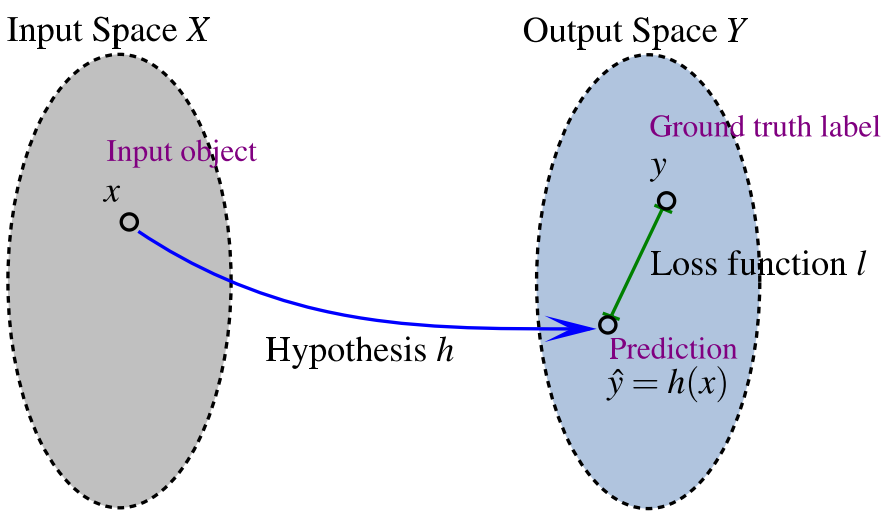
\includegraphics[scale=0.26]{gfx/descriminative_training}
\caption{Machine learning framework for Learning to Rank, obtained from Liu \cite{Liu2007}}
\label{fig:discriminative_training}
\end{figure}

Liu \cite{Liu2007} proposes a more narrow definition and only considers ranking methods to be a Learning to Rank method when it is \emph{feature based} and uses \emph{discriminative training}, in which the concepts \emph{feature based} and \emph{discriminative training} are itself defined as:
\begin{description}
\item[Feature Based]{means that all documents under investigation are represented by feature vectors. Those feature vectors reflect the relevance of the documents to the query, or the importance of the document in itself.}
\item[Discriminative Training]{means that the learning process can be well described by the four components of discriminative learning. That is, a Learning to Rank method has its own \emph{input space}, \emph{output space}, \emph{hypothesis space}, and \emph{loss function}, like the machine learning process described by Figure \ref{fig:discriminative_training}. \emph{Input space}, \emph{output space}, \emph{hypothesis space}, and \emph{loss function} are hereby defined as follows:
	\begin{description}
	\item[Input Space]{contains the objects under investigation. Usually objects are represented by feature vectors, extracted according to different applications.}
	\item[Output Space]{contains the learning target with respect to the input objects.}
	\item[Hypothesis Space]{defines the class of functions mapping the input space to the output space. The functions operate on the feature vectors of the input object, and make predictions according to the format of the output space.}
	\item[Loss Function]{in order to learn the optimal hypothesis, a training set is usually used, which contains a number of objects and their ground truth labels, sampled from the product of the input and output spaces. A loss function calculates the difference between the predictions $\hat{y}$ and the ground truth labels on a given set of data.
	\end{description}
	}
\end{description}


Figure \ref{fig:ltr_framework} shows how the machine learning process as described in Figure \ref{fig:discriminative_training} typically takes place in a ranking scenario. A set of queries $q_i$ with $n > i > 1$, the documents associated with these queries which are represented by feature vector $x_i$, and the relevant judgements of those documents $y_i$ are used together to train a model $h$. Model $h$ can after training be used to predict a ranking of the documents $y_i$, such the difference between the document rankings predicted by $h$ and the actual optimal rankings based on $y_i$ is minimal in terms of a loss function.
\begin{figure}[!h]
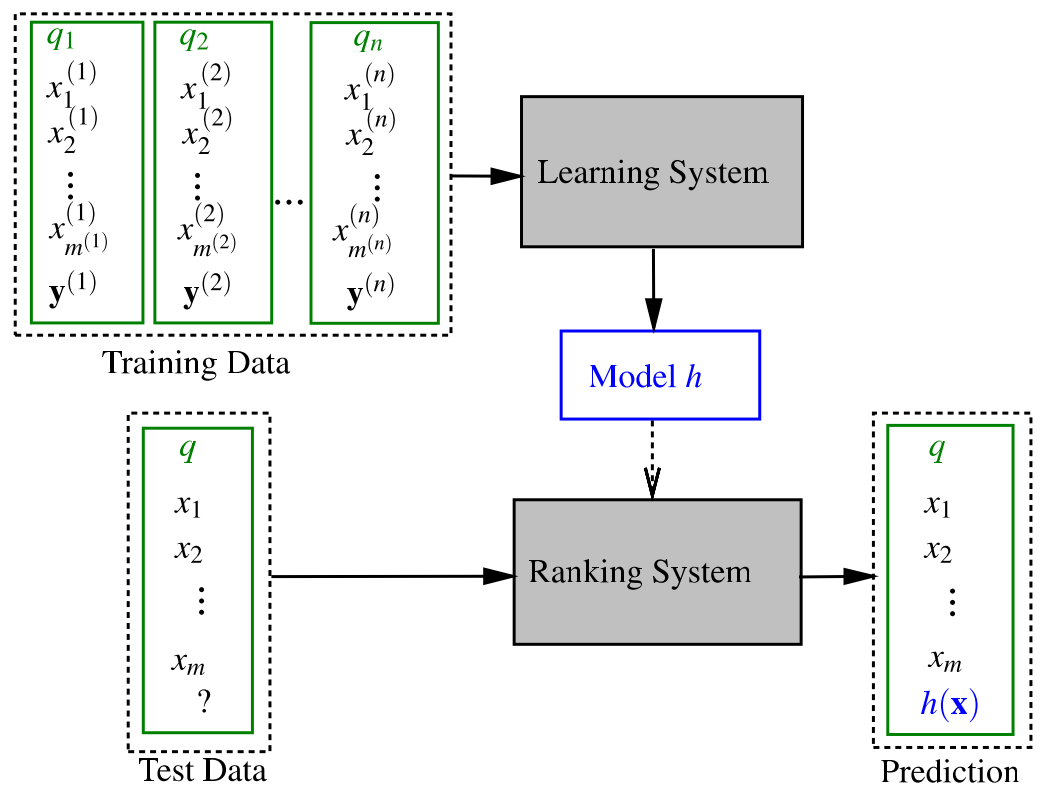
\includegraphics[scale=0.25]{gfx/ltr_framework}
\caption{A typical Learning to Rank setting, obtained from Liu \cite{Liu2007}}
\label{fig:ltr_framework}
\end{figure}\\

The predictions and the loss function might either be defined for:
\begin{enumerate}
\item the relevance of a single document
\item the classification of the most relevant document out of a document-pair
\item the ranking of documents directly
\end{enumerate}
\smallskip
These three approaches are in literature respectively labelled the pointwise approach, the pairwise approach and the listwise approach. These three approaches to Learning to Rank will be described in more detail in section \ref{sec:ltr_approaches}.

\section{How to evaluate a ranking}
\label{sec:how_to_evaluate_a_ranking}
Evaluation metrics have long been studied in the field of information retrieval. First in the form of evaluation of unranked retrieval sets and later, when the information retrieval field started focussing more on ranked retrieval, in the form of ranked retrieval evaluation. In this section several frequently used evaluation metrics for ranked results will be described.\\

No single evaluation metric that we are going to describe is indisputably better or worse than any of the other metrics. Different benchmarking settings have used different evaluation metrics. Metrics introduced in this section will be used in chapters \ref{chap:benchmark_results} and \ref{chap:cross_comparison} of this thesis to compare Learning to Rank methods in terms of ranking accuracy.
\subsection{Normalized Discounted Cumulative Gain}
Cumulative gain, or its successor discounted cumulative gain and normalized discounted cumulative gain, is one of the most widely used measures for effectiveness of ranking methods.
\subsubsection{Discounted Cumulative Gain}
There are two definitions of \ac{DCG} used in practice. \ac{DCG} at position $p$ was originally defined by J{\"a}rvelin and Kek{\"a}l{\"a}inen \cite{Jarvelin2002} as\\

$DCG_p = \sum\nolimits_{i=1}^p \frac{rel_i-1}{log_2(i+1)}$\\

with $rel_i$ the graded relevance of the result at position $i$. The idea is that highly relevant documents that appear lower in a search result should be penalized (discounted). This discounting is done by reducing the graded relevance  logarithmically proportional to the position of the result.\\

Burges et al. \cite{Burges2005} proposed an alternative definition of \ac{DCG} that puts stronger emphasis on document relevance\\

$DCG_p = \sum\nolimits_{i=1}^p \frac{2^{rel_i-1}}{log_2(i+1)}$\\

\subsubsection{Normalized Discounted Cumulative Gain}
\ac{NDCG} normalizes the \ac{DCG} metric to a value in the [0,1] interval by dividing by the \ac{DCG} value of the optimal rank. This optimal rank is obtained by sorting documents on relevance for a given query. The definition of \ac{NDCG} can be written down mathematically as\\

$nDCG_p = \frac{DCG_p}{IDCG_p}$\\

Table \ref{tab:example_calculation_NDCG} shows an example calculation for \ac{NDCG} for both the J{\"a}rvelin and Kek{\"a}l{\"a}inen \cite{Jarvelin2002} and Burges et al. \cite{Burges2005} version of \ac{DCG}.\\

\begin{table}[!h]
\begin{tabular}{llllllllllll}
 & \multicolumn{10}{c}{Rank} &  \\ 
\cline{2-11}
 & 1 & 2 & 3 & 4 & 5 & 6 & 7 & 8 & 9 & 10 & Sum \\ 
\hline
\hline
rel(i) & 10 & 7 & 6 & 8 & 9 & 5 & 1 & 3 & 2 & 4 &  \\
\hline
$\frac{2^{rel_i-1}}{log_2(i+1)}$ & 512 & 40.4 & 16 & 55.1 & 99.0 & 5.7 & 0.3 & 1.3 & 0.6 & 2.3 & 732.7 \\
\hline
$\frac{rel_i}{log_2(i+1)}$ & 10 & 4.42 & 3 & 3.45 & 3.48 & 1.78 & 0.33 & 0.95 & 0.6 & 1.16 & 29.17 \\  
\hline
\hline
optimal rank & 10 & 9 & 8 & 7 & 6 & 5 & 4 & 3 & 2 & 1 &  \\
\hline 
$\frac{2^{rel_i-1}}{log_2(i+1)}$ & 512 & 161.5 & 64 & 27.6 & 12.4 & 5.7 & 2.7 & 1.3 & 0.6 & 0.2 & 788.0 \\
\hline
$\frac{rel_i}{log_2(i+1)}$ & 10 & 5.68 & 4 & 3.01 & 2.32 & 1.78 & 1.33 & 0.95 & 0.6 & 0.29 & 29.96 \\   
\hline
 &  &  &  &  &  &  &  &  &  &  &  \\
 & \multicolumn{10}{c}{Burges \cite{Burges2005} et al. \ac{NDCG} = $\frac{732.7}{788.0} = 0.9298$} &  \\ 
  & \multicolumn{10}{c}{J{\"a}rvelin and Kek{\"a}l{\"a}inen \cite{Jarvelin2002} \ac{NDCG} = $\frac{29.17}{29.96} = 0.9736$} &  \\
\end{tabular}
\caption{Example calculation of \acs{NDCG}}
\label{tab:example_calculation_NDCG}
\end{table}

One limitation of \ac{NDCG} that it does not penalise for missing documents in the result set. \acl{NDCG} is often used with a fixed set size for the result set to mitigate the missing document problem. \ac{NDCG} with a fixed set size is often called \ac{NDCG}@k, where $k$ represents the set size.

\subsection{Expected Reciprocal Rank}
\ac{ERR} \cite{Chapelle2009} was designed based on the observation that \ac{NDCG} is based on the false assumption that the usefulness of a document at rank $i$ is independent of the usefulness of the documents at rank less than $i$. \ac{ERR} is based on the reasoning that users are likely to stop exploring the result list once they have found a document that satisfied their information need. The \ac{ERR} metric is defined as the expected reciprocal length of time that the user will take to find a relevant document. \ac{ERR} is formally defined as\\

$ERR = \sum\nolimits_{r=1}^n \frac{1}{r} \prod\nolimits_{i=1}^{r-1}(1-R_i)R_i$\\

where the product sequence part of the formula represents the chance that the user will stop at position $r$.\\
The algorithm to compute \ac{ERR} is shown in Listing \ref{alg:err}. The algorithm requires relevance grades $g_i$, $1 \le i \le n$ and mapping function $R$ that maps relevance grades to probability of relevance.

\LinesNumbered
\begin{algorithm}[H]
 $p \leftarrow 1, ERR \leftarrow 0$\\
 \For{$r\leftarrow 1$ \KwTo $n$}{
	$R \leftarrow R(g[r])$\\
	$ERR \leftarrow ERR + p * \frac{R}{r}$\\
	$p \leftarrow p * (1-R)$
 }
 Output $ERR$
 \caption{The algorithm for computation of the \acs{ERR} metric, obtained from \cite{Chapelle2009}}
 \label{alg:err}
\end{algorithm}

\subsection{Mean Average Precision}
\ac{AP} \cite{Zhu2004} is an often used binary relevance judgement based metric that can be seen as a trade-off between precision and recall that is defined as\\

$AP = \frac{\sum\nolimits_{k=1}^{n}Precision(k)*relevance(k)}{\text{number of relevant docs}}$\\

With $k$ being the positions in the result set between 1 and $n$. Table \ref{tab:example_calculation_AP} provides an example calculation of average precision where de documents at positions 1, 5, 6 and 8 in the ranking are relevant. The total number of available relevant documents in the document set \emph{R} is assumed to be seven.
\ac{MAP} is the average \ac{AP} for a set of queries.\\

$MAP = \frac{\sum\nolimits_{q=1}^{Q}AP(q)}{Q}$\\

\begin{table}
\begin{tabular}{lllllllllllll}
 & \multicolumn{10}{c}{Rank} &  & Sum \\ 
\cline{2-11}
 & 1 & 2 & 3 & 4 & 5 & 6 & 7 & 8 & 9 & 10 &  &  \\ 
\hline
$r_i$ & 1 & 0 & 0 & 0 & 1 & 1 & 0 & 1 & 0 & 0 &  &  \\ 
P@$i$ & 1 &  &  &  & 0.4 & 0.5 &  & 0.5 &  &  &  & 2.4 \\ 
\hline
 &  &  &  &  &  &  &  &  &  & \# of relevant docs & = & 7 \\ 
 &  &  &  &  &  &  &  &  &  & AP@10 & = & 0.34 \\ 
\end{tabular}
\caption{Average Precision example calculation.}
\label{tab:example_calculation_AP}
\end{table}

\section{Approaches to Learning to Rank}
\label{sec:ltr_approaches}
\subsection{Pointwise Approach}
The pointwise approach can be seen as the most straightforward way of using machine learning for ranking. Pointwise Learning to Rank methods directly apply machine learning methods to the ranking problem by observing each document in isolation. They can be subdivided in the following approaches:
	\begin{enumerate}
	\item regression-based, which estimate the relevance of a considered document using a regression model.
	\item classification-based, which classify the relevance category of the document using a classification model.
	\item ordinal regression-based, which classify the relevance category of the document using a classification model in such a way that the order of relevance categories is taken into account. 
	\end{enumerate}
Well-known algorithms that belong to the pointwise approach include McRank \cite{Li2007} and PRank \cite{Crammer2001}.
\subsection{Pairwise Approach}
Pointwise Learning to Rank methods have the drawback that they optimise real valued expected relevance, while evaluation metrics like \ac{NDCG} and \ac{ERR} are only impacted by a change in expected relevance when that change impacts a pairwise preference. The pairwise approach solves this drawback of the pointwise approach by regarding ranking as pairwise classification.\\

Aggregating a set of predicted pairwise preferences into the corresponding optimal rank is shown to be a NP-Hard problem \cite{Feldman2012}. An often used solution to this problem is to upper bound the number of classification mistakes by an easy to optimise function \cite{Bartlett2006}.\\

Well-known pairwise Learning to Rank algorithms include FRank \cite{Tsai2007}, GBRank \cite{Zheng2007}, LambdaRank \cite{Burges2006}, RankBoost \cite{Freund2003}, RankNet \cite{Burges2005}, Ranking \acs{SVM} \cite{Herbrich1999b,Joachims2002}, and SortNet \cite{Rigutini2008}.
\subsection{Listwise Approach}
Listwise ranking optimises the actual evaluation metric. The learner learns to predict an actual ranking itself without using an intermediate step like in pointwise or pairwise Learning to Rank. The main challenge in this approach is that most evaluation metrics are not differentiable. \ac{MAP}, \ac{ERR} and \ac{NDCG} are non-differentiable, non-convex and discontinuous functions, what makes them very hard to optimize.\\

Although the properties of \ac{MAP}, \ac{ERR} and \ac{NDCG} are not ideal for direct optimisation, some listwise approaches do focus on direct metric optimisation \cite{Yue2007, Taylor2008, Chapelle2010}. Most listwise approaches work around optimisation of the non-differentiable, non-convex and discontinuous metrics by optimising surrogate cost functions that mimic the behaviour of \ac{MAP}, \ac{ERR} or \ac{NDCG}, but have nicer properties for optimisation.\\

Well-known algorithms that belong to the listwise approach include AdaRank \cite{Xu2007}, BoltzRank \cite{Volkovs2009}, ListMLE \cite{Xia2008}, ListNet \cite{Cao2007}, RankCosine \cite{Qin2008}, SmoothRank \cite{Chapelle2010}, SoftRank \cite{Taylor2008}, \acs{SVM}$^{map}$ \cite{Yue2007}.

\section{Cross-validation experiments}
\label{sec:cross_validation}
A cross-validation experiment \cite{kohavi1995}, sometimes called rotation estimation, is an experimental set-up for model evaluation where the data is split into $k$ chunks of approximately equal size, called \emph{folds}. One of the folds is used as validation set, one of the folds is used as test set, and the rest of the $k - 2$ folds are used as training data. This procedure is repeated $k$ times, such that each fold is once used for validation, once as test set, and $k - 2$ times as training data. The performance can be measured in any model evaluation metric, and is averaged over the model performances on each of the folds. The goal of cross-validation is to define a data set to test the model in the training phase, in order to limit the problem of overfitting.\\

Cross-validation is one of the most frequently used model evaluations methods in the field of Machine Learning, including the Learning to Rank subfield. Often, folds in a cross-validation are created in a \emph{stratified} manner, meaning that the folds are created in such a way that the distributions of the target variable are approximately identical between the folds.

\section{An introduction to the MapReduce programming model}
MapReduce \cite{Dean2004} is a programming model invented at Google, where users specify a \emph{map} function that processes a key/value pair to generate a set of intermediate key/value pairs, and a \emph{reduce} function that merges all intermediate values associated with the same intermediate key. This model draws its inspiration from the field of functional programming, where \emph{map} and \emph{reduce} are commonly used functions.\\

This combination of the \emph{map} and \emph{reduce} functions allows for parallel computation. In the \emph{map} phase parallel computation can be performed by simply splitting the input data after a certain number of bytes, where each worker nodes performs the user-specified \emph{map}-function on its share of the data. Before the \emph{reduce} phase these intermediate answers of the different worker nodes are transformed in such a way that they are grouped by key value, this is called the shuffle-phase. After the shuffle-phase, the user-defined \emph{reduce}-function is applied to each group of key/value pairs in the reduce phase. Since the key/value pairs are already grouped by key in the shuffle phase, this \emph{reduce}-function can be applied to a group of key/value pairs on any of the worker nodes.\\
%\addtocontents{toc}{\protect\clearpage} % <--- just debug stuff, ignore
%\include{multiToC} % <--- just debug stuff, ignore for your documents
\part{Related Work}
\section{Literature study characteristics}
The literature research is performed by using the bibliographic databases Scopus and Web of Science with the following search query: \emph{("learning to rank" OR "learning-to-rank" OR "machine learned ranking") AND ("parallel" OR "distributed")}. An abstract based manual filtering step is applied where I filter those results that actually use the \emph{parallel} or \emph{distributed} terms in context to the \emph{learning to rank}, \emph{learning-to-rank} or \emph{machine learned ranking}. Studies focusing on efficient query evaluation instead of efficient model training are likely to meet all criteria listed. As a last step I will filter out studies based on the whole document that only focus on efficient query evaluation and not on parallel or distributed learning of ranking functions.\\

on Scopus the defined search query resulted in 65 documents. Only 14 of those documents used \emph{large scale}, \emph{parallel} or \emph{distributed} terms in context to the \emph{learning to rank}, \emph{learning-to-rank} or \emph{machine learned ranking}. 10 out of those 14 documents focussed on parallel or distributed learning of ranking functions.\\

The defined search query resulted in 16 documents on Web of Science. Four of those documents were also present in the set of 65 documents found using Scopus, leaving 61 unique documents. Only four of those 61 documents used \emph{large scale}, \emph{parallel} or \emph{distributed} terms in context to the \emph{learning to rank}, \emph{learning-to-rank} or \emph{machine learned ranking}, none of them focussed on parallel or distributed learning of ranking functions.\\

On Google Scholar the defined search query resulted in 3300 documents. We evaluate the first 300 search results.\\

Section \ref{sec:lit_descr} describe the approaches on parallel or distributed Learning-to-Rank found in literature.
\section{Literature description}
\label{sec:lit_descr}
Different approaches to parallelising Learning-to-Rank can be identified in literature. The following subsections describe the related work in the field categorised by approach.

\subsection{Parallelising Learning-to-Rank through ensemble learning}
Schapire proved in 1990 that a strong model can be generated by combining weak models through a procedure that he called boosting \cite{Schapire1990}. The invention of the boosting method resulted in an increasing focus in machine learning research on methods to combine multiple weak models, which are called ensemble learning methods. Well-known ensemble methods include gradient boosting \cite{Friedman2001}, bagging \cite{Breiman1996}, AdaBoost \cite{Freund1997} and stacked generalisation (stacking) \cite{Wolpert1992}.\\

Ensemble methods can be used to parallelise learning methods by training the weak models in the ensemble on different nodes. In the Learning-to-Rank field parallelisation of model training through ensemble learning is frequently achieved using decision tree learners and often using the boosting ensemble method, jointly called \acf{GBDT}. \ac{GBDT}'s are shown to be able to achieve good accuracy in a Learning-to-Rank setting when used in a pairwise \cite{Zheng2007} or listwise \cite{Chen2008} setting.

\subsubsection{Gradient Boosting}
Gradient Boosting \cite{Friedman2001} is an ensemble learning method in which multiple weak learners are iteratively added together into one ensemble model in such a way that new models focus more on those data instances that were misclassified before.\\

Kocsis et al. \cite{Kocsis2013} propose way to train multiple weak learners in parallel by extending those models that are likely to yield a good model when combined through boosting. Authors showed through theoretical analysis that the proposed algorithm asymptotically achieve equal performance to regular gradient boosting. \ac{GBDT} models could be trained in parallel using their BoostingTree algorithm.\\

Tyree et al. \cite{Tyree2011} describe a way of parallelising \ac{GBDT} models for Learning-to-Rank where the boosting step is still executed sequentially, instead the construction of the regression trees themselves are parallelised. The parallel decision tree building is based on Ben-Haim and Yom-Tov's work on parallel construction of decision trees for classification \cite{Ben-Haim2010}. Decision trees are build layer-by-layer where the calculations needed for building each new layer in the tree are divided over the nodes using a master-worker paradigm. The data is partitioned of the workers, who compress their share into histograms and send these to the master. The master uses those histograms to approximate the split and build the next layer. The master than communicates this new layer to the workers who can use this new layer to compute new histograms. this process is repeated until the tree depth limit is reached. The tree construction algorithm parallelised with described master-worker method is \ac{CART} \cite{Breiman1984}. Speed-up experiments on the LETOR and the Yahoo! Learning to Rank challenge data sets were performed. This parallel \ac{CART}-tree building approach showed speed-up of up to 42x on shared memory machines and up to 25x on distributed memory machines.\\

Ye et al. \cite{Ye2009} described how to implement the stochastic \ac{GBDT} model in a parallel manner using both MPI and Hadoop. Stochastic \ac{GBDT} differs from regular \ac{GBDT} models by using stochastic gradient boosting instead of regular gradient boosting. Stochastic gradient boosting is a minor alteration to regular gradient boosting that, at each iteration of the algorithm, trains a base learner on a sub-sample of the training set that is drawn at random without replacement \cite{Friedman2002}. Experiments showed the Hadoop implementation to result into too expensive communication cost to be useful. Authors believed that these high communication costs were a result of the communication intensive implementation that was not well suited for the MapReduce paradigm. The MPI approach proved to be successful and obtained near linear speed-ups.

\subsubsection{Boosting wrapped in Bagging}
Some approaches combine both boosting and bagging. Bagging \cite{Breiman1996}, also called bootstrap aggregating, is a ensemble learning method in which $m$ training sets $D_1..D_m$ are constructed from the training set $D$ by uniformly sampling data items from $D$ with replacement. The bagging method is parallelisable by training each $D_i$ with $i \in \{1..m\}$ on a different node.\\

Pavlov et al. \cite{Pavlov2010} from Yandex were the first to propose a boosting-wrapped-in-bagging approach, which they called BagBoo. The boosting step itself is not parallelisable, but the authors state that learning a short boosted sequence on a single node is still a do-able task.

Ganjisaffar \cite{Ganjisaffar2011b} proposed a pairwise boosting-wrapped-in-bagging model called BL-MART, in contrast to BagBoo which is a pointwise model. BL-MART adds a bagging step to the LambdaMART \cite{Wu2008} ranking model, a model that uses the Gradient Boosting \cite{Friedman2002} ensemble method combined with regression tree weak learners. In contract to BagBoo, BL-MART is limited in the number of trees. An experiment on the TD2004 dataset resulted in 4500 trees using BL-MART while 1.1 million trees were created with the BagBoo model.

\subsubsection{Stacked generalisation}
A \ac{DSN} is a processing architecture developed from the field of \emph{Deep Learning}, that uses the \ac{MSE} loss function that is easily optimisable. \ac{DSN} is based on the stacked generalization ensemble learning method \cite{Wolpert1992}, an approach where several learning models are stacked on top of each other in such a way that the output of a model is used as one of the input features of models higher up in the stack. Each layer in the stack learns has the task of learning the weights of the inputs of that layer. The close-form constraints between input and output weights allow the input weight matrices to be estimated in a parallel manner.\\

\subsection{Low complexity Learning-to-Rank}
Designing Learning-to-Rank algorithms with low time complexity for training is another approach towards large scale Learning-to-Rank. Pahikkala et al. \cite{Pahikkala2009} describe a pairwise \ac{RLS} type of ranking function, RankRLS, with time complexity $\mathcal{O}(n^3+n^2m)$, with $n$ the number of features and $m$ the number of training documents. The RankRLS ranking function showed ranking performance similar to RankSVM on the BioInfer corpus \cite{Pyysalo2007}, a corpus for information extraction in the biomedical domain.

\subsection{CCRank}
Wang et al. \cite{Wang2011a,Wang2011b} propose a parallel evolutionary algorithm based on \ac{CC}, a type of evolutionary algorithm. The \ac{CC} algorithm is capable of directly optimizing non-differentiable functions, as \ac{nDCG}, in contrary to many optimization algorithms.  the divide-and-conquer nature of the \ac{CC} algorithm enables parallelisation. CCRank showed an increase in both accuracy and efficiency on the LETOR 4.0 benchmark dataset compared to the baselines. It must be stated however that the increased efficiency was achieved through speed-up and not scale-up. Two reasons have been identified for not achieving linear scale-up with CCRank: 1) parallel execution is suspended after each generation to perform combination in order to produce the candidate solution, 2) Combination has to wait until all parallel tasks have finished, which may spend different running time.
\subsection{Parallel ListNet using Spark}
Shukla et al. \cite{Shukla2012} explored the parallelisation of the well-known ListNet Learning-to-Rank method using Spark. Spark is a parallel computing model that is designed for cyclic data flows which makes it more suitable for iterative algorithms. Spark is incorporated into Hadoop since Hadoop 2.0. The Spark implementation of ListNet showed near a linear training time reduction.
\subsection{nDCG-Annealing}
Karimzadeghan et al. \cite{Karimzadehgan2011} proposed a method using Simulated Annealing along with the Simplex method for its parameter search. This method directly optimises the often non-differentiable Learning-to-Rank evaluation metrics like \ac{nDCG} and \ac{MAP}. The authors successfully parallelised their method in the MapReduce paradigm using Hadoop. The approach showed to be effective on both the LETOR 3.0 dataset and their own dataset with contextual advertising data. Unfortunately their work does not directly report on the speed-up obtained by parallelising  with Hadoop, but it is mentioned that further work needs to be done to effectively leverage parallel execution.

\subsection{Distributed Stochastic Gradient Descent}
Long et al. \cite{Long2012} describe special case of their pairwise cross-domain factor Learning-to-Rank method using distributed optimization of \ac{SGD} based on Hadoop MapReduce. Parallelisation of the \ac{SGD} optimization algorithm was performed using the MapReduce based method described by  Zinkevich et al. \cite{Zinkevich2010} has been used. Real world data from Yahoo! has been used to show that the model is effective. Unfortunately the speed-up obtained by training their model in parallel is not reported.
\subsection{FPGA-based LambdaRank}
Yan et al. \cite{Yan2009,Yan2010,Yan2011,Yan2012} described the development and incremental improvement of a \ac{SIMD} architecture \ac{FPGA} designed to run the Neural Network based LambdaRank Learning-to-Rank algorithm. This architecture achieved a 29.3X speed-up compared to the software implementation when evaluated on data from a commercial search engine. The exploration of \ac{FPGA} for Learning-to-Rank showed other advantages of the \ac{FPGA} approach next to faster model training. In their latest publication \cite{Yan2012} the \ac{FPGA} based LambdaRank implementation showed it could achieve up to 19.52X power efficiency and 7.17X price efficiency for query processing compared to Intel Xeon servers currently used at the commercial search engine.
\subsection{GPGPU for Learning-to-Rank}
De Sousa et al. \cite{DeSousa2012} proposed a \ac{GPGPU} approach using the \ac{GPU} both learning the ranking function and for query processing, thereby improving both training time and query time. An association rule based Learning-to-Rank approach proposed by \cite{Veloso2008} has been implemented using the \ac{GPU} in such a way that the set of rules van be computed in parallel, in different threads, for each document. A speed-up of 127X in query processing time is reported based on evaluation on the LETOR dataset. The speed-up achieved at learning the ranking function was unfortunately not stated.

\subsection{Alternating Direction Method of Multipliers}
Duh et al. \cite{Duh2011} propose the use of \ac{ADMM} for the Learning-to-Rank task. \ac{ADMM} is a general optimization method that solves problems of the form
\begin{alignat*}{2}
\text{minimize }   &  f(x) + g(x) \\
\text{subject to } &  Ax + Bz = c
\end{alignat*}
by updating $x$ and $z$ in an alternating fashion. It holds the nice properties that it can be executed in parallel and that it allows for incremental model updates without full retraining. Duh et al. \cite{Duh2011} show how to use \ac{ADMM} to train a RankSVM model in parallel. Experiments showed the \ac{ADMM} implementation to achieve a 13.1x training time speed-up on 72 workers, compared to training on a single worker.\\

Another \ac{ADMM} Learning-to-Rank based approach was proposed by Boyd et al. \cite{Boyd2012}. Boyd et al. \cite{Boyd2012} implemented an \ac{ADMM} based Learning-to-Rank method in Pregel \cite{Malewicz2010}, a parallel computation framework for graph computations. No experimental results on parallelisation speed-up were reported on this Pregel based approach.
\subsection{Distributed Hyper-parameter Tuning using MapReduce}
Ganjisaffar et al. \cite{Ganjisaffar2011, Ganjisaffar2011b} observed that long training times are often a result of training many models for hyperparameter optimisation. Grid search is the \emph{de facto} standard of hyperparameter optimisation and is simply an exhaustive search through a manually specified subset of hyperparameter combinations. The authors show how to perform parallel grid search on MapReduce clusters, which is easy because grid search is an embarrassingly parallel method as hyperparameter combinations are mutually independent. They apply their grid search on MapReduce approach in a Learning-to-Rank setting to train a LambdaMART \cite{Wu2008} ranking model, a model that uses the Gradient Boosting \cite{Friedman2002} ensemble method combined with regression tree weak learners. Experiments showed that the solution scales linearly in number of hyperparameter combinations. However, the risk of overfitting grows overwhelmingly as the number of hyperparameter combinations grow, even when validation sets grow large.
\subsection{Distributed LambdaRank}
Svore and Burges \cite{Svore2010,Svore2012} designed two approaches to train the LambdaMART \cite{Wu2008} model in a distributed manner. Their first approach is applicable in case the whole training set fits in main memory on every node, in that case the tree split computations of the regressions trees in the LambdaMART tree ensemble are split and the data is not. The second approach distributes the training data and corresponding training computations and is therefore scalable to high amounts of training data. Both approaches achieves a six times speed-up over LambdaMART on 32 nodes compared to a single node.
\subsection{Learning-to-Rank with Bregman Divergences and Monotone Retargeting}
Acharyya et al. \cite{Acharyya2012} propose a Learning-to-Rank method searches for an order preserving transformation (\emph{monotone retargeting}) of the target scores that is easier for a regressor to fit. This approach is based on the observation that it is not necessary to fit scores exactly, since the evaluation is dependent on the order and not on the pointwise predictions themselves.\\

Bregman divergences are a family of distance-like functions that do not satisfy symmetry nor the triangle inequality. A well-known member of the class of Bregman divergences is Kullback-Leibler divergence, also known as \emph{information gain}.\\

Acharyya et al. \cite{Acharyya2012} defined a parallel algorithm that optimises a Bregman divergence function as surrogate of \ac{nDCG} that is claimed to be well suited for implementation of a \ac{GPGPU}. No experiments on speed-up have been performed.
\subsection{Parallel robust Learning-to-Rank}
Robust learning \cite{Huber1981} is defined as the task to lean a model in the presence of outliers. Yun et al. describe a \cite{Yun2014} robust Learning-to-Rank model called RoBiRank that has the additional advantage that it is executable in parallel. Their RoBiRank model uses parameter expansion to linearise a surrogate loss function, after which the elements of the linear combination can be divided over the available nodes. The Parameter expansion trick was proposed by Gopal and Yang \cite{Gopal2013}, who originally proposed it for multinomial logistic regression. Unfortunately, no speed-up experiments were mentioned for the RoBiRank method, since Yun et al. focussed their research more on robust ranking than on parallel ranking. The only reference to performance of RoBiRank in terms of speed is the statement that its training time on a computing cluster is comparable to the more efficient implementation by Lee and Lin \cite{Lee2014} of a linear kernel RankSVM \cite{Herbrich1999, Joachims2002}.
\ctparttext{This part describes benchmark characteristics like collection size and features and gives an overview of the performance of different Learning-to-Rank methods. Performance differences for a given Learning-to-Rank method are explained in terms of differences in benchmark characteristics. This section is concluded with a selection of Learning-to-Rank methods to include in the experiments.}
\part{Benchmark results}
\chapter{Yahoo! Learning to Rank Challenge}
Yahoo's observation that all existing benchmark datasets were too small to draw reliable conclusions, especially in comparison with datasets used in commercial search engines, prompted Yahoo to release two internal datasets from Yahoo! search. The Yahoo! Learning to Rank Challenge\cite{Chapelle2011a} is a public Learning-to-Rank competition which took place from March to May 2010, with the goal to promote the datasets and encourage the research community to develop new Learning-to-Rank algorithms.\\

The Yahoo! Learning to Rank Challenge consists of two tracks that uses the two datasets respectively: a standard Learning-to-Rank track and a transfer learning track where the goal was to learn a specialized ranking function that can be used for a small country by leveraging a larger training set of another country. For this experiment I will only look at the standard Learning-to-Rank dataset because transfer learning is a separate research area that is not included in this thesis.\\
\begin{table}[!h]
\begin{tabular}{l|lll}
 & Train & Validation & Test \\ 
 \hline
Queries & 19,994 & 2,994 & 6,983 \\ 
Documents & 473,134 & 71,083 & 165,660 \\ 
Features & 519 & - & - \\ 
\end{tabular}
\caption{Yahoo! Learning to Rank Challenge dataset characteristics, as described in the challenge overview paper\cite{Chapelle2011a}}
\label{tab:yahoo_characteristics}
\end{table}\\
Both \ac{nDCG} and \ac{ERR} are measured as performance metrics, but the final standings of the challenge were based on the \ac{ERR} values. Model validation on the Learning-to-Rank methods participating in the challenge is performed using a train/validation/test-set split following the characteristics shown in Table \ref{tab:yahoo_characteristics}. Competitors could train on the training set and get immediate feedback on their performance on the validation set. The test set performance is used to create the final standings and is only measured after the competition has ended to avoid overfitting on the test set. The large number of documents, queries and features compared to other benchmark datasets makes the Yahoo! Learning to Rank Challenge dataset interesting. Yahoo did not provide detailed feature descriptions to prevent competitors to get detailed insight in the characteristics of the Yahoo data collection and features used at Yahoo. Instead high level descriptions of feature categories are provided. The following categories of features are described in the challenge overview paper\cite{Chapelle2011a}:\\
\begin{description}
\item[Web graph]{Quality and popularity metrics of web documents, e.g. PageRank\cite{Page1999}}.
\item[Document statistics]{Basic document statistics such as the number of words and url characteristics.}
\item[Document classifier]{Results of various classifiers on the documents. These classifiers amongst others include: spam, adult, language, main topic, and quality classifiers.}
\item[Query]{Basic query statistics, such as the number of terms, query frequency, and click-through rate.}
\item[Text match]{Textual similarity metrics between query and document. Includes \ac{TF-IDF}, BM25\cite{Robertson2009} and other metrics for different sections of the document.}
\item[Topical matching]{These features go beyond similarity at word level and compute similarity on topic level. For example by classifying both the document and the query in a large topical taxonomy.}
\item[Click]{Click-based user feedback.}
\item[External references]{Document meta-information such as Delicious\footnote{https://delicious.com/} tags}
\item[Time]{Document age and historical in- and outlink data that might help for time sensitive queries.}
\end{description}

\section{Results}
Figure \ref{fig:yahoo_results} shows the top five participants in the Yahoo! Learning to Rank Challenge in terms of ERR score. The top five participants all used decision trees and ensemble methods. Burges et al\cite{Burges2011} created a linear combination ensemble of eight LambdaMART\cite{Burges2010}, two LambdaRank and two Logistic Regression models. Gottschalk and Vogel used a combination of RandomForest models and \ac{GBDT} models. Pavlov and Brunk used a regression based model using the BagBoo\cite{Pavlov2010} ensemble technique, which combines bagging and boosting. Sorokina used a similar combination of bagging and boosting that is called Additive Groves\cite{Sorokina2007}.\\

The challenge overview paper states as one of the lessons of the challenge that the simple baseline \ac{GBDT} model performed very well with a small performance gap to the complex ensemble submissions at the top of the table.

\begin{table}
\begin{tabular}{l|p{6.3cm}|l}
 & Authors & ERR \\
 \hline 
1 & Burges et al (Microsoft Research) & 0.46861 \\ 
2 & Gottschalk (Activision Blizzard) \& Vogel (Data Mining Solutions) & 0.46786 \\ 
3 & Parakhin (Microsoft) & 0.46695 \\ 
4 & Pavlov \& Brunk (Yandex Labs) & 0.46678 \\ 
5 & Sorokina (Yandex Labs) & 0.46616 \\ 
\end{tabular}
\caption{Final standings of the Yahoo! Learning to Rank Challenge, as presented in the challenge overview paper\cite{Chapelle2011a}}
\label{fig:yahoo_results}
\end{table}



\chapter{Yandex Internet Mathematics competition}

\section{Results}



\chapter{LETOR}
The LETOR benchmark set was first released by Microsoft Research Asia in April 2007 to solve the absence of a experimental platform for Learning-to-Rank at that time. LETOR has been updated several times since: LETOR 2.0 was released at the end of 2007, LETOR 3.0 in December 2008 and LETOR 4.0 in July 2009. The original LETOR benchmark collection\cite{Liu2007b} as released in 2007 contained two data sets: the OHSUMED collection and the .gov collection.\\

The OHSUMED collection is a subset of the medical publication database MEDLINE and contains medical publications from 270 journals that were published between 1987 and 1991. The .gov collection is a web crawl obtained in January 2002, which was used for the TREC web track in 2003 and 2004. Tables \ref{tbl:features_gov} and \ref{tbl:features_ohsumed} provide the descriptions of the features of the .gov and the OHSUMED collections respectively.\\

Different query sets exists for the .gov corpus. Those query sets can be categorized in \emph{topic distillation} (TD), \emph{named page finding} (NP) and \emph{home page finding} (HP). With query sets available from both the TREC 2003 and 2004 conferences there are six query sets in total: TD2003, TD2004, NP2003, NP2004, HP2003 and HP2004.\\

The evaluation metrics used are \ac{nDCG} and \ac{MAP}. The \emph{winning number} metric is defined as the number of other algorithms that it can beat over all of the seven datasets (six .gov sets + OHSUMED). The LETOR organisation implemented and evaluated several well-known Learning-to-Rank algorithms themselves and in addition gathers and publications and results of new algorithms evaluated on the LETOR benchmark. The baseline Learning-to-Rank algorithms evaluated by the organisation are:
\begin{description}
\item[pointwise]{\leavevmode
	\begin{itemize}
	\item Linear regression
	\end{itemize}}
\item[pairwise]{\leavevmode
	\begin{itemize}
	\item RankingSVM\cite{Herbrich1999,Joachims2002}
	\item RankBoost\cite{Freund2003}
	\item FRank\cite{Tsai2007}
	\end{itemize}}
\item[listwise]{\leavevmode
	\begin{itemize}
	\item ListNet\cite{Cao2007}
	\item AdaRank-MAP\cite{Xu2007}
	\item AdaRank-nDCG\cite{Xu2007}
	\item SVMMAP\cite{Yue2007} 
	\end{itemize}}
\end{description} 
\begin{table}[!h]
\scalebox{0.87}{
\begin{tabular}{p{0.29cm}|p{7.26cm}||p{0.29cm}|p{9.55cm}}
 \textbf{ID} & \textbf{Feature Description} & \textbf{ID} & \textbf{Feature Description}\\ 
 \hline
1 & \ac{TF} of body					& 36& LMIR.JM of body\\
2 &	\ac{TF} of anchor				& 37& LMIR.JM of anchor\\
3 & \ac{TF} of title				& 38& LMIR.JM of title\\
4 & \ac{TF} of \ac{URL}				& 39& LMIR.JM of \ac{URL}\\
5 & \ac{TF} of whole document		& 40& LMIR.JM of whole document\\

6 & \ac{IDF} of body 				& 41& Sitemap based term propagation\\
7 & \ac{IDF} of anchor 				& 42& Sitemap based score propagation\\
8 & \ac{IDF} of title 				& 43& Hyperlink based score propagation: weighted in-link\\
9 & \ac{IDF} of \ac{URL} 			& 44& Hyperlink based score propagation: weighted out-link\\
10& \ac{IDF} of whole document 		& 45& Hyperlink based score propagation: uniform out-link\\

11& \ac{TF-IDF} of body 			& 46& Hyperlink based feature propagation: weighted in-link\\
12& \ac{TF-IDF} of anchor 			& 47& Hyperlink based feature propagation: weighted out-link\\
13& \ac{TF-IDF} of title 			& 48& Hyperlink based feature propagation: uniform out-link\\
14& \ac{TF-IDF} of \ac{URL}			& 49& HITS authority\\
15& \ac{TF-IDF} of whole document	& 50& HITS hub\\

16& Document length of body			& 51& PageRank\\
17& Document length of anchor		& 52& HostRank\\
18& Document length of title		& 53& Topical PageRank\\
19& Document length of \ac{URL}		& 54& Topical HITS authority\\
20& Document length of whole document	& 55& Topical HITS hub\\

21& BM25 of body					& 56& In-link number\\
22& BM25 of anchor					& 57& Out-link number\\
23& BM25 of title					& 58& Number of slashes in \ac{URL}\\
24& BM25 of \ac{URL}				& 59& Length of \ac{URL}\\
25& BM25 of whole document			& 60& Number of child page\\

26& LMIR.ABS\cite{Zhai2001} of body	& 61& BM25 of extracted title\\
27& LMIR.ABS of anchor				& 62& LMIR.ABS of extracted title\\
28& LMIR.ABS of title				& 63& LMIR.DIR of extracted title\\
29& LMIR.ABS of \ac{URL}			& 64& LMIR.JM of extracted title\\
30& LMIR.ABS of whole document\\

31& LMIR.DIR of body\\
32& LMIR.DIR of anchor\\
33& LMIR.DIR of title\\
34& LMIR.DIR of \ac{URL}\\
35& LMIR.DIR of whole document\\
\end{tabular}
}
\caption{Features of the LETOR .GOV dataset, obtained from Qin et al\cite{Qin2010}}
\label{tbl:features_gov}
\end{table}

\begin{table}[!h]
\scalebox{0.87}{
\begin{tabular}{p{0.29cm}|p{6.88cm}||p{0.29cm}|p{6.90cm}}
 \textbf{ID} & \textbf{Feature Description} & \textbf{ID} & \textbf{Feature Description}\\ 
 \hline
1 & $\sum\nolimits_{q_i \in q \cap d}c(q_i, d)$ of title					& 24&  $\sum\nolimits_{q_i \in q \cap d}c(q_i,d)\cdot log(\frac{|C|}{df(q_i)})$ of abstract\\
2 &	$\sum\nolimits_{q_i \in q \cap d}log(c(q_i, d)+1)$ of title				& 25& $\sum\nolimits_{q_i \in q \cap d} log(\frac{c(q_i,d)}{|d|}) \cdot \frac{|C|}{c(q_i,C)}+1$ of abstract\\
3 & $\sum\nolimits_{q_i \in q \cap d}\frac{c(q_i,d)}{|d|}$ of title				& 26& BM25 of abstract\\
4 & $\sum\nolimits_{q_i \in q \cap d}log(\frac{c(q_i,d)}{|d|}+1)$ of title				& 27& $log($BM25$)$ of abstract\\
5 & $\sum\nolimits_{q_i \in q \cap d}log(\frac{|C|}{df(q_i)})$ of title		& 28& LMIR.DIR of abstract\\

6 & $\sum\nolimits_{q_i \in q \cap d}log(log(\frac{|C|}{df(q_i)}))$ of title 				& 29& LMIR.JM of abstract\\
7 & $\sum\nolimits_{q_i \in q \cap d}log(\frac{|C|}{c(q_i,C)}+1)$ of title 				& 30& LMIR.ABS of abstract\\
8 & $\sum\nolimits_{q_i \in q \cap d}log(\frac{c(q_i,d)}{|d|} \cdot \frac{|C|}{df(q_i)}+1)$ of title 				& 31& $\sum\nolimits_{q_i \in q \cap d}c(q_i, d)$ of title + abstract\\
9 & $\sum\nolimits_{q_i \in q \cap d}c(q_i,d)\cdot log(\frac{|C|}{df(q_i)})$ of title 			& 32&	$\sum\nolimits_{q_i \in q \cap d}log(c(q_i, d)+1)$ of title + abstract\\
10& $\sum\nolimits_{q_i \in q \cap d} log(\frac{c(q_i,d)}{|d|}) \cdot \frac{|C|}{c(q_i,C)}+1$ of title		& 33& $\sum\nolimits_{q_i \in q \cap d}\frac{c(q_i,d)}{|d|}$ of title + abstract\\

11& BM25 of title 			& 34& $\sum\nolimits_{q_i \in q \cap d}log(\frac{c(q_i,d)}{|d|}+1)$ of title + abstract\\
12& $log($BM25$)$ of title 			& 35& $\sum\nolimits_{q_i \in q \cap d}log(\frac{|C|}{df(q_i)})$ of title + abstract\\
13& LMIR.DIR of title 			& 36& $\sum\nolimits_{q_i \in q \cap d}log(log(\frac{|C|}{df(q_i)}))$ of title + abstract\\
14& LMIR.JM of title			& 37& $\sum\nolimits_{q_i \in q \cap d}log(\frac{|C|}{c(q_i,C)}+1)$ of title + abstract\\
15& LMIR.ABS of title	& 38& $\sum\nolimits_{q_i \in q \cap d}log(\frac{c(q_i,d)}{|d|} \cdot \frac{|C|}{df(q_i)}+1)$ of title + abstract\\

16& $\sum\nolimits_{q_i \in q \cap d}c(q_i, d)$ of abstract		& 39& $\sum\nolimits_{q_i \in q \cap d}c(q_i,d)\cdot log(\frac{|C|}{df(q_i)})$ of title + abstract\\
17& $\sum\nolimits_{q_i \in q \cap d}log(c(q_i, d)+1)$ of abstract		& 40& $\sum\nolimits_{q_i \in q \cap d} log(\frac{c(q_i,d)}{|d|}) \cdot \frac{|C|}{c(q_i,C)}+1$ of title + abstract\\
18& $\sum\nolimits_{q_i \in q \cap d}\frac{c(q_i,d)}{|d|}$ of abstract		& 41& BM25 of title + abstract\\
19& $\sum\nolimits_{q_i \in q \cap d}log(\frac{c(q_i,d)}{|d|}+1)$ of abstract		& 42& $log($BM25$)$ of title + abstract\\
20& $\sum\nolimits_{q_i \in q \cap d}log(\frac{|C|}{df(q_i)})$ of abstract	& 43& LMIR.DIR of title + abstract\\

21& $\sum\nolimits_{q_i \in q \cap d}log(log(\frac{|C|}{df(q_i)}))$ of abstract					& 44& LMIR.JM of title + abstract\\
22&  $\sum\nolimits_{q_i \in q \cap d}log(\frac{|C|}{c(q_i,C)}+1)$ of abstract					& 45& LMIR.ABS of title + abstract\\
23& $\sum\nolimits_{q_i \in q \cap d}log(\frac{c(q_i,d)}{|d|} \cdot \frac{|C|}{df(q_i)}+1)$ of abstract					& & \\
\end{tabular}
}
\caption{Features of the LETOR OHSUMED dataset, obtained from Qin et al\cite{Qin2010}}
\label{tbl:features_ohsumed}
\end{table}
\section{Results}
\begin{figure}[!h]
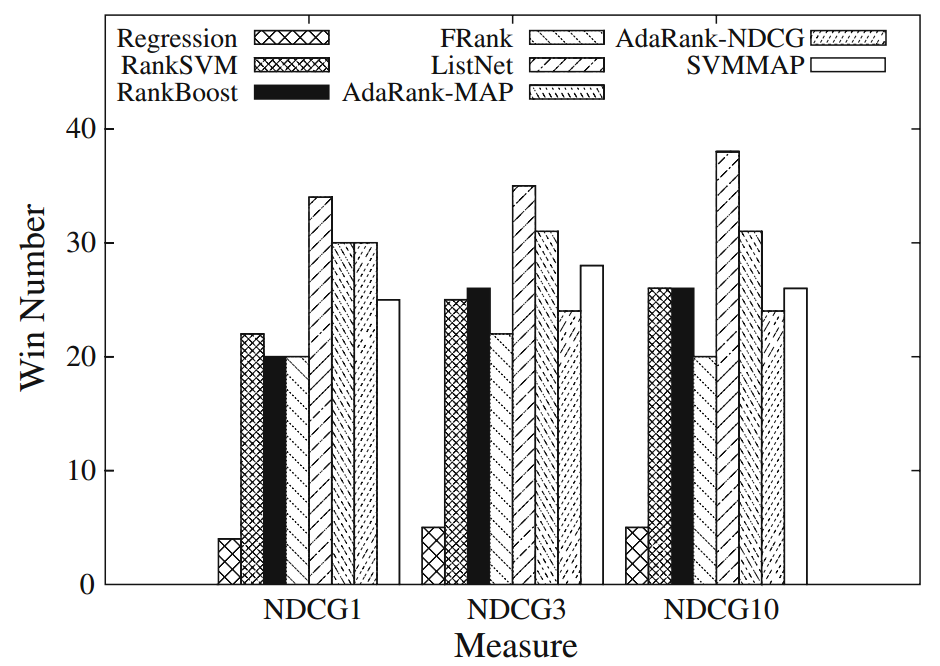
\includegraphics[scale=0.30]{gfx/ndcg_winning_number}
\caption{Comparison across the seven datasets in LETOR by \ac{nDCG}, obtained from Qin et al\cite{Qin2010}}
\label{fig:ndcg_winning_number}
\end{figure}

\begin{figure}[!h]
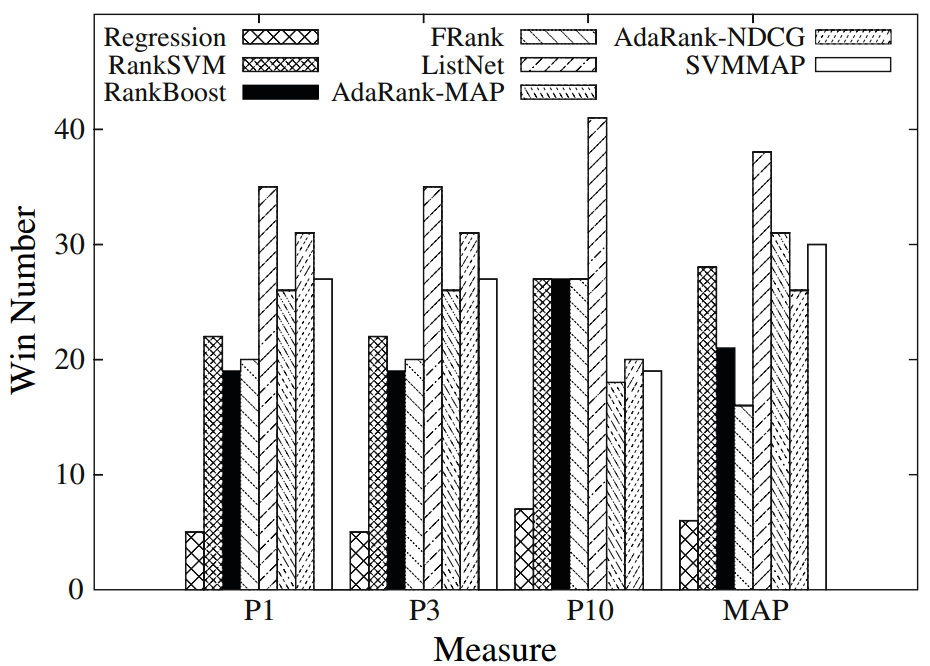
\includegraphics[scale=0.30]{gfx/map_winning_number}
\caption{Comparison across the seven datasets in LETOR by \ac{MAP}, obtained from Qin et al\cite{Qin2010}}
\label{fig:map_winning_number}
\end{figure}


\chapter{MSLR-WEB10k/MSLR-WEB30k}
Contrary to the Yahoo! Learning to Rank Challenge dataset, the MSLR-WEB30k provides detailed feature descriptions. The MSLR-WEB30k dataset however contains no proprietary features but only features that are commonly used in the research community.
\section{Results}

\chapter{Selecting Learning-to-Rank methods}
The Accuracies of the Learning-to-Rank methods described in the preceding chapters must only be compared within the benchmark and not between benchmarks for the following reasons:
\begin{enumerate}
\item Differences in feature sets between data sets detract from fair comparison
\item Although the \ac{nDCG} definition is unambiguous, Busa-Fekete et al\cite{Busa-Fekete2012} found that \ac{nDCG} evaluation tools of benchmark data sets produced different scores
\end{enumerate}
\ctparttext{Algorithms and details of the well-performing Learning-to-Rank methods as selected in the aforegoing part are presented and explained in this part.}
\part{Selected Learning-to-Rank methods}
Algorithms and details of the well-performing Learning-to-Rank methods as selected in the afore-going part are presented and explained in this part.

\section{ListNet}
ListNet \cite{Cao2007} is a listwise ranking function whose loss function is not directly related to information retrieval evaluation metrics. ListNet's loss function is defined using a probability distribution on permutations. Probability distributions on permutations have been a research topic within the field of probability theory and has been extensively researched. One of the most well-known permutation probability distributions in the field, the Plackett-Luce model \cite{Plackett1975,Luce1959}, is used in ListNet. The Plackett-Luce model defines the probability of all possible permutations $\pi$, given all document ranking scores $S$, as shown in Equation \ref{eq:plackett_luce}.
\begin{equation}
P(\pi|S) = \prod\limits_{j=1}^{m}\frac{\phi(s_{\pi^{-1}(j)})}{\sum\nolimits_{u=1}^{m}\phi(s_{\pi^{-1}(u)})}
\label{eq:plackett_luce}
\end{equation}
ListNet uses Gradient Descent to optimise neural network such that its Cross Entropy loss compared to the Plackett-Luce distribution over the ground truth is minimal. Note that some sources, including Liu \cite{Liu2007}, describe ListNet as using KL divergence as loss function. KL divergence and Cross-entropy are however identical up to an additive constant when comparing distribution $q$ against a fixed reference distribution $p$, since the cross-entropy definition can be formulated as in Equation \ref{eq:cross_entropy}.
\begin{equation}
H(p,q) = H(p) + D_{KL}(p||q)
\label{eq:cross_entropy}
\end{equation}
where $H(p)$ is the entropy of $p$ and $D_{KL}(p||q)$ is the Kullback-Leibler divergence of $q$ from $p$.\\

\noindent Equation \ref{eq:gradient_descent} describes the gradient descent step to minimise loss function $L(y^{(i)},z^{(i)}(f_\omega))$ with respect to parameter $\omega$. 
\begin{equation}
\Delta\omega = \frac{\partial L(y^{(i)},z^{(i)}(f_\omega))}{\partial \omega} = - \sum_{\forall g \in \mathscr{G}_k}\limits\frac{\partial P_{z^{(i)}(f_\omega)}(g)}{\partial \omega}\frac{P_{y^{(i)}}(g)}{P_{z^{(i)}(f_\omega)}(g)}
\label{eq:gradient_descent}
\end{equation}

\noindent Algorithm \ref{alg:listnet} shows the pseudo-code of the ListNet training phase.\\
\LinesNumbered
\begin{algorithm}[H]
 \KwData{training data \{$(x^{(1)},y^{(1)}),(x^{(2)},y^{(2)}),...,(x^{(m)},y^{(m)})$\}}
 \KwIn{number of iterations $T$ and learning rate $\eta$}
 Initialize parameter $\omega$\\
 \For{$t\leftarrow 1$ \KwTo $T$}{
 	\For{$i\leftarrow 1$ \KwTo $m$}{
 		Input $x^{(i)}$ of query $q^{(i)}$ to Neural Network and compute score list $z^{(i)}(f_\omega)$ with current $\omega$.\\
 		Compute gradient $\Delta\omega$ using Eq. (\ref{eq:gradient_descent}).\\
 		Update $\omega = \omega - \eta \times \Delta\omega$.
 	}
 }
 Output Neural Network model $\omega$.
 \caption{Learning algorithm of ListNet, obtained from \cite{Cao2007}}
 \label{alg:listnet}
\end{algorithm}

\section{SmoothRank}
SmoothRank \cite{Chapelle2010} is a listwise ranking method that directly optimises an information retrieval evaluation measure by smoothing, that is, approximating the rank position. In this section I will use \ac{nDCG} for illustration of SmoothRank, but the same procedure can also be applied to \ac{MAP} or any other information retrieval measure. The smoothing function used in SmoothRank based on the softmax activation function \cite{Bridle1990} that is often used in neural networks, which is formally defined as shown in Equation \ref{eq:softmax_algorithm}.
\begin{equation}
p_i = \frac{e^{f_i/\sigma}}{\sum\nolimits_{j=1}^{m}e^{f_j/\sigma}}
\label{eq:softmax_algorithm}
\end{equation}

where $\sigma$ is the smoothing parameter. Chapelle et al \cite{Chapelle2010} apply the softmax activation function to the \ac{nDCG} formula and thereby introduce a soft version of indicator variable $h_{i,j}$ as formulated in Equation \ref{eq:soft_ndcg}.

\begin{equation}
h_{i,j} = e^{-\frac{(f(x_i))-(f(x_{d(j)}))^2}{\sigma}}\Big/\sum\nolimits_{k=1}^{m}e^{-\frac{(f(x_k))-f(x_{d(j)})^2}{\sigma}}
\label{eq:soft_ndcg}
\end{equation}

It can be shown that the derivative of the smoothed \ac{nDCG} version shown in Equation \ref{eq:soft_ndcg} and the smoothed versions of other \ac{IR} metrics can be calculated in $\mathcal{O}(m^2)$, which enable fast gradient descent optimisation. The optimisation step in SmoothRank uses the nonlinear conjugate gradient method  with Polak-Ribiere update \cite{Shewchuk1994}, which is a type of gradient descent method. The optimisation method is prone to local optima, which is alleviated by adding a good starting point and regulariser.\\

The starting point in SmoothRank is set to either the solution of a simple linear regression, or alternatively to the solution of Rank\acs{SVM}. Since this starting point is expected to already be a good solution, a regulariser term is added to the SmoothRank objective function to prevent the solution from deviating to much from the starting point. The regularised smooth objective function is formulated as $\lambda||w-w_0||^2$ where $\lambda$ is a hyperparameter tuned on the validation set, and $w_0$ is the starting point solution.\\

The choice of the smoothing parameter $\sigma$ in Equation \ref{eq:soft_ndcg} is important, because a too small value makes the function more non-smooth and therefore harder to optimise, while a too large value results in a optimisation function that substantially differs from the optimal rankings. SmoothRank uses an annealing method where the optimisation procedure starts with a large $\sigma$ and iteratively reduces it by dividing it by 2 at each step. Algorithm \ref{alg:smoothrank} shows the algorithm that summarises all steps of the SmoothRank method.\\
\LinesNumbered
\begin{algorithm}[H]
 Find an initial solution $w_0$ (by regression of Rank\acs{SVM}).\\
 Set $w = w_0$ and $\sigma$ to a large value.\\
 \While{Stopping condition not satisfied}{
 	 Starting from $w$, minimize by non-linear conjugate gradient descent:
 	 $\lambda||w-w_0||^2 - \sum\nolimits_{q}A_q(w,\sigma)$\\
 	 $\sigma = \sigma/2$
 }
 \caption{Learning algorithm of SmoothRank, obtained from \cite{Chapelle2010}}
 \label{alg:smoothrank}
\end{algorithm}

\section{FenchelRank}
FenchelRank \cite{Lai2013} learning method that addresses the sparse Learning-to-Rank problem, which is the problem of learning a ranking function with only a few non-zero coefficients with respect to the input features. FenchelRank is based on the theory of Fenchel Duality \cite{Rifkin2007} and uses the genetic algorithm framework proposed by Shalev-Shwartz and Singer \cite{Shalev-Shwartz2010}.

FenchelRank optimises the objective function shown in Equation \ref{eq:pairwise_l1_loss} that is equivalent to the standard $\ell_1$-norm regularised pairwise loss function.

\begin{equation}
\min_w G(w) = \min_w I_{||w||_{1} \le 1}(w) + \frac{r^2}{p} \sum\limits_{i=1}^{p}\max(0,\frac{1}{r}-(Kw)_i)^2
\label{eq:pairwise_l1_loss}
\end{equation}

The objective function in Equation \ref{eq:pairwise_l1_loss} is not differentiable everywhere because of its $\ell_1$-norm regularisation term.

Let $D(w) = -G(w)$, then the objective function stated in \ref{eq:pairwise_l1_loss} can be rewritten as shown in Equation \ref{eq:fenchel_dual}.
\begin{equation}
\max_w D(w) = \max_w I_{||w||_{1} \le 1}(w) - \frac{r^2}{p} \sum\limits_{i=1}^{p}\max(0,\frac{1}{r}-(Kw)_i)^2
\label{eq:fenchel_dual}
\end{equation}


\LinesNumbered
\begin{algorithm}[H]
 \KwData{pairwise training data matrix $K$}
 \KwIn{desired accuracy $\epsilon$, maximum number of iterations $T$ and the radius $r$ of the $\ell1$ ball.}
 Initialize: $w_1$ = $0_m$\\
 \For{$t\leftarrow 1$ \KwTo $T$}{
 	//check if the early stopping criterion is satisfied\\
 	\If{$||g_{t}||_{\infty} + \langle d_{t}, -Kw_{t} \rangle \le \epsilon$}{
 	// Here $d_{t} = \nabla f^{*}(-Kw_{t}) = \frac{\partial f^{*}(-Kw)}{\partial(Kw)}|w=w_{t}$ and $g_{t} = d_{t}^{T}K$\\
 	return $w_{t}$ as ranking predictor $w$
 	}
 //greedily choose a feature to update\\
 Choose $j_{t} = \argmax_{j}|(g_t)_j)|$\\
 //compute an appropriate step size\\
 Let $\mu_t = \argmax_{0 \le \mu_{t} \le 1} D((1-\mu_{t})w_{t} + \mu_{t}\sign((g_{t})_{j_{t}})e^{j_{t}})$\\
 //update the model with the chosen feature and step size\\
 Update $w_{t+1}=(1-\mu_{t})w_{t} + \mu_{t}\sign((g_{t})j_{t})e^{j_{t}}$
 }
 return $w_{T}$ as ranking predictor for $w$
 \caption{Learning algorithm of FenchelRank, obtained from \cite{Lai2013}}
 \label{alg:fenchelrank}
\end{algorithm}
\section{FSMRank}

\section{LRUF}
Learning automaton.
\ctparttext{Describes implementation details of the Learning-to-Rank algorithm parallel implementations in HDInsight that are either Hadoop, Microsoft Azure, or HDInsight and are not part of the algorithm specification itself.}
\part{Implementation}
\label{chap:implementation}
The first section of this chapter will briefly discuss the HDInsight platform, the Hadoop ecosystem components offered by HDInsight and, in this regard, the Hadoop components used for implementation of the algorithms described in Chapter \ref{chap:ltr_methods}. The second section of this chapter describes a Java framework that handles the joint components needed for MapReduce Learning to Rank computation that are independent of the Learning to Rank model. The subsequent sections describe the implementation details of specific Learning to Rank models.

\section{Architecture}
Ranking algorithms consist of a sequence of operations on the input data which are often, but not always, of iterative nature. Apache Pig \cite{Olston2008} will be used to implement the sequence of operation on the input data. Pig Latin, the data processing language that runs on Apache Pig, designed based on the observation that the traditional MapReduce paradigm is too low-level and rigid, and holds the middle between the declarative style of SQL and the procedural style of MapReduce. The Apache Pig system translates Pig Latin into MapReduce plans that are executed over Hadoop. The choice to implement the Learning to Rank algorithms in Pig Latin allow more focus on the data operations and less focus on low-level implementation details compared to native Hadoop MapReduce. Furthermore, it allows us to rely on Apache Pig to create efficient MapReduce plans out of the Pig Latin code which lowers the implementation-dependent factor of the experiments.\\

\subsection{Storing Input Data for HDInsight Processing}
Azure HDInsight supports both the traditional \ac{HDFS} as described by Shvacko et al. \cite{Shvachko2010}, as well as Microsoft's own \ac{WASB} storage solution. Blob storage decouples the storage from the HDInsight Hadoop cluster; it enables safe deletion of a HDInsight cluster without losing data, as data is not solely stored on the cluster itself, but also on a separate storage that is not cluster-dependent. Azure \ac{WASB} storage allows the user to select one of their data centre for storage. \ac{WASB} storage in the West Europe region (located in Amsterdam) will be used for storage, as this data centre is located close to where the experiments are executed.

\subsection{Microsoft Azure HDInsight Job submission}
Microsoft offers a scalable and on-demand Hadoop service with HDInsight, that enables Hadoop services for those not able to make the required investments for their own cluster. The latest HDInsight of HDInsight available at the time of writing, HDInsight 3.1, runs the Hortonworks distribution of Hadoop version 2.4. HDInsight 3.1 offers multiple ways of submitting Hadoop jobs to a HDInsight cluster, described in Table \ref{tbl:hdinsight_endpoints}.\\

\begin{table}
\centering
\begin{tabular}{p{4.2cm}p{2.6cm}p{5.5cm}}\toprule
Job submission method & Type & Description \\
\midrule
Powershell & Powershell scripts & The Azure module for Windows PowerShell enables direct submission of Hadoop jobs through PowerShell cmdlets.\\
C\# API & C\# API & A wrapper API is offered to submit Hadoop MapReduce jobs directly from C\# code.\\
HiveServer/HiveServer2 & REST endpoint & Apache Hive \cite{Thusoo2009} is an open-source data warehousing solution on top of Hadoop, that supports processing of a SQL-like declarative language called HiveQL. HiveServer and its successor HiveServer 2 are REST endpoints that allow remote submission of HiveQL queries.\\
Oozie & REST endpoint & Apache Oozie \cite{Islam2012} is a workflow scheduler to manage Apache Hadoop jobs. Oozie enables users to specify Directed Acyclical Graphs of action, where each action is specified in either MapReduce or Pig.\\
WebHCat/Templeton & REST endpoint & WebHCat, formerly known as Templeton, is a REST API for HCatalog, a table and storage management layer for Hadoop. WebHCat allows users to use either Apache Pig, Apache MapReduce or Apache Hive for data processing.\\	
\bottomrule
\end{tabular}
\caption{HDInsight REST endpoints for job submission}
\label{tbl:hdinsight_endpoints}
\end{table}

Oozie and WebHCat/Templeton are the two methods for job submission in Table \ref{tbl:hdinsight_endpoints} that both 1) support Apache Pig jobs, and 2) Can be used from within Java code. Below the necessary procedures for job submission from Oozie as well as from WebHCat will be sketched.\\

% TODO: Stuk over werkzaamheden framework uitbreiden: uitlezen resultaten (evaluatieresultaten + doorgeven tussenresultaten (die tweede wellicht later in het document pas introduceren))
Fold handling  in a cross-validation experiment is the process of loading the correct data folds for training, validation and testing in the multiple rounds that the cross-validation experiment consists of. Fold handling is a task that needs to be taken care of regardless of the ranking model that is being evaluated. Given that most ranking models are of an iterative nature, the task of iteration handling is also a task that need to be done for most models. Iteration handling and fold handling are procedures in which the same steps are repeated for each iteration or cross-validation round respectively. Pig Latin, however, has no support for loops which are needed to perform iteration handling and fold handling. Since iteration handling and fold handling are tasks that need to be addressed for each ranking model and that cannot be solved with Pig, we create a framework that takes care of both iteration and fold handling and generates the Pig Latin code for the current iteration and fold. The aim of this framework is to let implementations of ranking models focus solely on implementing the sequential steps of one iteration of the algorithm, while the framework arranges that 1) these sequential steps are performed iteratively and 2) these sequential steps are performed on the multiple training folds of data. This framework that handles folding and iterations will be implemented in Java and will work such that fold- and iteration dependent parts of the Pig code will be generated dynamically by the Java framework after which the Pig job will be sent to the cluster.\\

Another responsibility of the framework is to handle communication between multiple Pig jobs within a single iteration of a Learning to Rank algorithm. The framework enables reading the result of a Pig job from \ac{WASB} storage which can then be used as parameter within a subsequent Pig job. An example of this is a Pig implementation of gradient descent, where a first Pig job might calculate gradients and writes them to storage, after which the framework assists in reading the gradients from storage and allows them to be used as input parameters of a second Pig job that calculates new feature weights based on its gradient parameter and a predetermined step size.\\

\begin{table}
\centering
\begin{tabular}{p{5cm}p{5cm}}\toprule
Job submission procedure for Apache Oozie & Job submission procedure for WebHCat/Templeton \\
\midrule
1. Let the framework build the Pig job dynamically. & 1. Let the framework build the Pig job dynamically.\\
2. Encapsulate the Pig job in an Oozie workflow. & 2. Submit the Pig job through the WebHCat/Templeton REST API.\\
3. Upload the Oozie workflow to HDFS storage. & \\
4. Execute the Oozie workflow through the Oozie REST API. & \\
\bottomrule
\end{tabular}
\caption{Comparison of Oozie and WebHCat job submission procedures}
\label{tbl:oozie_templeton}
\end{table}

Table \ref{tbl:oozie_templeton} shows how Oozie job submission is more complex then for the case of dynamically generated jobs than WebHCat/Templeton. Oozie is more fitting for static Hadoop jobs that require a workflow consisting of a sequence of Pig and MapReduce jobs mixed together, but is a lesser fit for our situation. Templeton will be used for submission of the Pig jobs, as the HDInsight version that was available at the start of the implementation did not yet support WebHCat.

\subsection{ListNet}
The following sections describe the Pig jobs that form the three independent parts of the ListNet ranking model: 1) Preprocessing, 2) Training (this includes evaluation over the validation set) and 3) Testing (evaluation over the test set). 
\subsubsection{Preprocessing}
The preprocessing phase consists of two separate Pig jobs. The first Pig job determines the minimum and the maximum values per feature in the training set. The second Pig job rescales each feature of the train, validation and test datasets using the following formula for rescaling:
\begin{equation}
x^{'} = \frac{x-min(x)}{max(x)-min(x)}
\end{equation}
This rescaling procedure sets the values of all features to be within range $[0,1]$.\\

The first Pig job:\\
\begin{minipage}{\linewidth}
\begin{lstlisting}
REGISTER [path prefix]/lib/*.jar;
TRAIN = LOAD '[path prefix]/input/[dataset name]/Fold[fold number]/train.txt' USING PigStorage(' ');
TRAIN_STD = FOREACH TRAIN GENERATE flatten(udf.util.ToStandardForm(*));
TRAIN_STD_BY_QUERY = GROUP TRAIN_STD BY $1 PARALLEL [available reducers];
MIN_MAX = FOREACH TRAIN_STD_BY_QUERY GENERATE flatten(udf.util.GetMinMax(*));
MIN_MAX_GRPD = GROUP MIN_MAX ALL;
MIN_MAX_FIN = FOREACH MIN_MAX_GRPD GENERATE flatten(udf.util.CombineMinMax(*));
STORE MIN_MAX_FIN INTO 'minmax[fold number]';
\end{lstlisting}
\end{minipage}

The minimum and maximum values per feature stored in MIN\_MAX\_FIN can now be read from \ac{HDFS} and used within the Java framework by using the Windows Azure Storage library. The second Pig job uses these minimum and maximum values by parametrising the \ac{UDF} that performs the rescaling transformation, udf.util.ScaleFeatures(), with the minimum and maximum feature values.\\

\begin{table}
\centering
\begin{tabular}{p{5cm}p{8cm}}\toprule
UDF & Description \\
\midrule
udf.util.ToStandardForm() & Transforms the data set into the standard form of relevance label in first column followed by feature values. Strips data of any other columns, if present.\\
udf.util.GetMinMax() & Extracts the minimum and maximum value per feature, for the documents of a single query.\\
udf.util.CombineMinMax() & Combines outputs of the udf.util.GetMinMax() UDF for each query into globally minimum and maximum feature values.\\
\bottomrule
\end{tabular}
\caption{Description of preprocessing User Defined Functions (1/2)}
\label{tbl:preprocessing_udfs_1}
\end{table}

The second Pig job:\\
\begin{minipage}{\linewidth}
\begin{lstlisting}
REGISTER [path prefix]/lib/*.jar;
TRAIN = LOAD '[path prefix]/input/[dataset name]/Fold[fold number]/train.txt' USING PigStorage(' ');
VALIDATE = LOAD '[path prefix]/input/[dataset name]/Fold[fold number]/vali.txt' USING PigStorage(' ');
TEST = LOAD '[path prefix]/input/[dataset name]/Fold[fold number]/test.txt' USING PigStorage(' ');
TRAIN_STD = FOREACH TRAIN GENERATE flatten(udf.util.ToStandardForm(*));
VALIDATE_STD = FOREACH VALIDATE GENERATE flatten(udf.util.ToStandardForm(*));
TEST_STD = FOREACH TEST GENERATE flatten(udf.util.ToStandardForm(*));
DEFINE ScaleFeatures udf.util.ScaleFeatures('[array with minimum and maximum feature values]');
TRAIN_SCA = FOREACH TRAIN_STD GENERATE flatten(ScaleFeatures(*));
VALIDATE_SCA = FOREACH VALIDATE_STD GENERATE flatten(ScaleFeatures(*));
TEST_SCA = FOREACH TEST_STD GENERATE flatten(ScaleFeatures(*));
STORE TRAIN_SCA INTO 'train_sca[fold number]' USING BinStorage();
STORE VALIDATE_SCA INTO 'validate_sca[fold number]' USING BinStorage();
STORE TEST_SCA INTO 'test_sca[fold number]' USING BinStorage();
\end{lstlisting}
\end{minipage}

\begin{table}
\centering
\begin{tabular}{p{5cm}p{8cm}}\toprule
UDF & Description \\
\midrule
udf.util.ToStandardForm() & See Table \ref{tbl:preprocessing_udfs_1} for description.\\
udf.util.ScaleFeatures() & Uses the minimum and maximum feature values with which it is parametrised perform the following rescaling transformation to the features: $x^{'} = \frac{x-min(x)}{max(x)-min(x)}$.\\
\bottomrule
\end{tabular}
\caption{Description of preprocessing User Defined Functions (2/2)}
\label{tbl:preprocessing_udfs_2}
\end{table}

\subsubsection{Training}
The training stage, like the preprocessing stage, consists of two separate Pig jobs. The first Pig job calculates the Cross Entropy loss on training data of the current model and calculates the gradients for the next model update. The second Pig job is an internal validation step that validates the model on the validation set by calculating \ac{nDCG}@k.\\

The first Pig job:\\
\begin{minipage}{\linewidth}
\begin{lstlisting}
REGISTER [path prefix]/lib/*.jar;
DEFINE QueryLossGradient udf.listnet.QueryLossGradient('[feature dimensionality of data set]');
DEFINE ExpRelOurScores udf.listnet.ExpRelOurScores('[neural network weights & iteration number]');
[FIRST TRAINING ITERATION:]
	TRAIN_SCA = LOAD 'train_sca[fold number]/*' USING BinStorage();
	TR_BY_QUERY = GROUP TRAIN_SCA BY $1 PARALLEL [number of avaiable reducers];
	TR_EXP_REL_SCORES = FOREACH TR_BY_QUERY GENERATE flatten(ExpRelOurScores(TRAIN_SCA));
	STORE TR_EXP_REL_SCORES INTO 'tr_exp_rel_scores-f[fold number]' USING BinStorage();
[SUBSEQUENT TRAINING ITERATIONS:]
	TR_EXP_REL_SCORES = LOAD 'tr_exp_rel_scores-f[fold number]/*' USING BinStorage();
	TR_EXP_REL_SCORES = FOREACH TR_EXP_REL_SCORES GENERATE flatten(ExpRelOurScores(*)) PARALLEL [number of available reducers];
TR_QUERY_LOSS_GRADIENT = FOREACH TR_EXP_REL_SCORES GENERATE flatten(QueryLossGradient(*)) PARALLEL [number of available reducers];
TR_QUERY_LOSS_GRADIENT_GRPD = GROUP TR_QUERY_LOSS_GRADIENT ALL;
TR_LOSS_GRADIENT = FOREACH TR_QUERY_LOSS_GRADIENT_GRPD GENERATE flatten(udf.listnet.MultiSum(*));
STORE TR_LOSS_GRADIENT INTO 'tr_loss_gradient-f[fold number]i[iteration number]';
\end{lstlisting}
\end{minipage}

\begin{table}
\centering
\begin{tabular}{p{5cm}p{8cm}}\toprule
UDF & Description \\
\midrule
udf.listnet.QueryLossGradient() & Calculates the Cross Entropy loss for a query and calculates the gradients per feature based on this query.\\
udf.listnet.ExpRelOurScores() & Calculates the predicted relevance label of a query based on the current model weights and transforms this following the transformation $x -> e^{x}$. In case the current iteration is the first iteration, the same transformation is applied to the ground truth relevance label.\\
udf.listnet.MultiSum() & Calculates aggregated loss and feature gradients by summing the per-query losses and per-query feature gradients.\\
\bottomrule
\end{tabular}
\caption{Description of training User Defined Functions (1/2)}
\label{tbl:training_udfs_1}
\end{table}

The second Pig job of the training stage validates the performance of the model weights that were trained in the first Pig job on the validation data set.\\

The second Pig job:\\
\begin{minipage}{\linewidth}
\begin{lstlisting}
REGISTER [path prefix]/lib/*.jar;
DEFINE Ndcg udf.util.Ndcg('[neural network weights & NDCG cut-off parameter]');
[FIRST TRAINING ITERATION:]
	VALIDATE_SCA = LOAD 'validate_sca[fold number]/*' USING BinStorage();
	VA_BY_QUERY = GROUP VALIDATE_SCA BY $1 PARALLEL [number of available reducers];
	STORE VA_BY_QUERY INTO 'va_by_query-f[fold number]' USING BinStorage();
[SUBSEQUENT TRAINING ITERATIONS:]
	VA_BY_QUERY = LOAD 'va_by_query-f[fold number]/*' USING BinStorage();
NDCG = FOREACH VA_BY_QUERY GENERATE Ndcg(*);
NDCG_GRPD = GROUP NDCG ALL;
AVG_NDCG = FOREACH NDCG_GRPD GENERATE AVG(NDCG);
STORE AVG_NDCG INTO 'avg_ndcg-f[fold number]i[iteration number]';
\end{lstlisting}
\end{minipage}

\begin{table}
\centering
\begin{tabular}{p{5cm}p{8cm}}\toprule
UDF & Description \\
\midrule
udf.util.Ndcg() & Calculates \ac{nDCG}@k for a query.\\
\bottomrule
\end{tabular}
\caption{Description of training User Defined Functions (2/2)}
\label{tbl:training_udfs_2}
\end{table}

\subsubsection{Testing}
The testing stage tests the best model found in the training iterations, selected on validation set \ac{nDCG}@k (as calculated in the second Pig job of the training stage), by calculating the \ac{nDCG}@k of this model on the test set.\\

Test stage Pig job:\\
\begin{minipage}{\linewidth}
\begin{lstlisting}
REGISTER [path prefix]/lib/*.jar;
TEST_SCA = LOAD 'test_sca[fold number]/*' USING BinStorage();
TE_BY_QUERY = GROUP TEST_SCA BY $1 PARALLEL [number of available reducers];
DEFINE Ndcg udf.util.Ndcg('[neural network weights & NDCG cut-off parameter]');
NDCG = FOREACH TE_BY_QUERY GENERATE Ndcg(*);
NDCG_GRPD = GROUP NDCG ALL;
AVG_NDCG = FOREACH NDCG_GRPD GENERATE AVG(NDCG);
STORE AVG_NDCG INTO 'avg_ndcg';
\end{lstlisting}
\end{minipage}

\subsection{SmoothRank}
\part{Results \& Discussion}
This chapter describes the results of the running time measurements of the cluster and baseline implementations as described in \ref{chap:implementation}.
\section{ListNet}
Figure
\begin{figure}
\centering
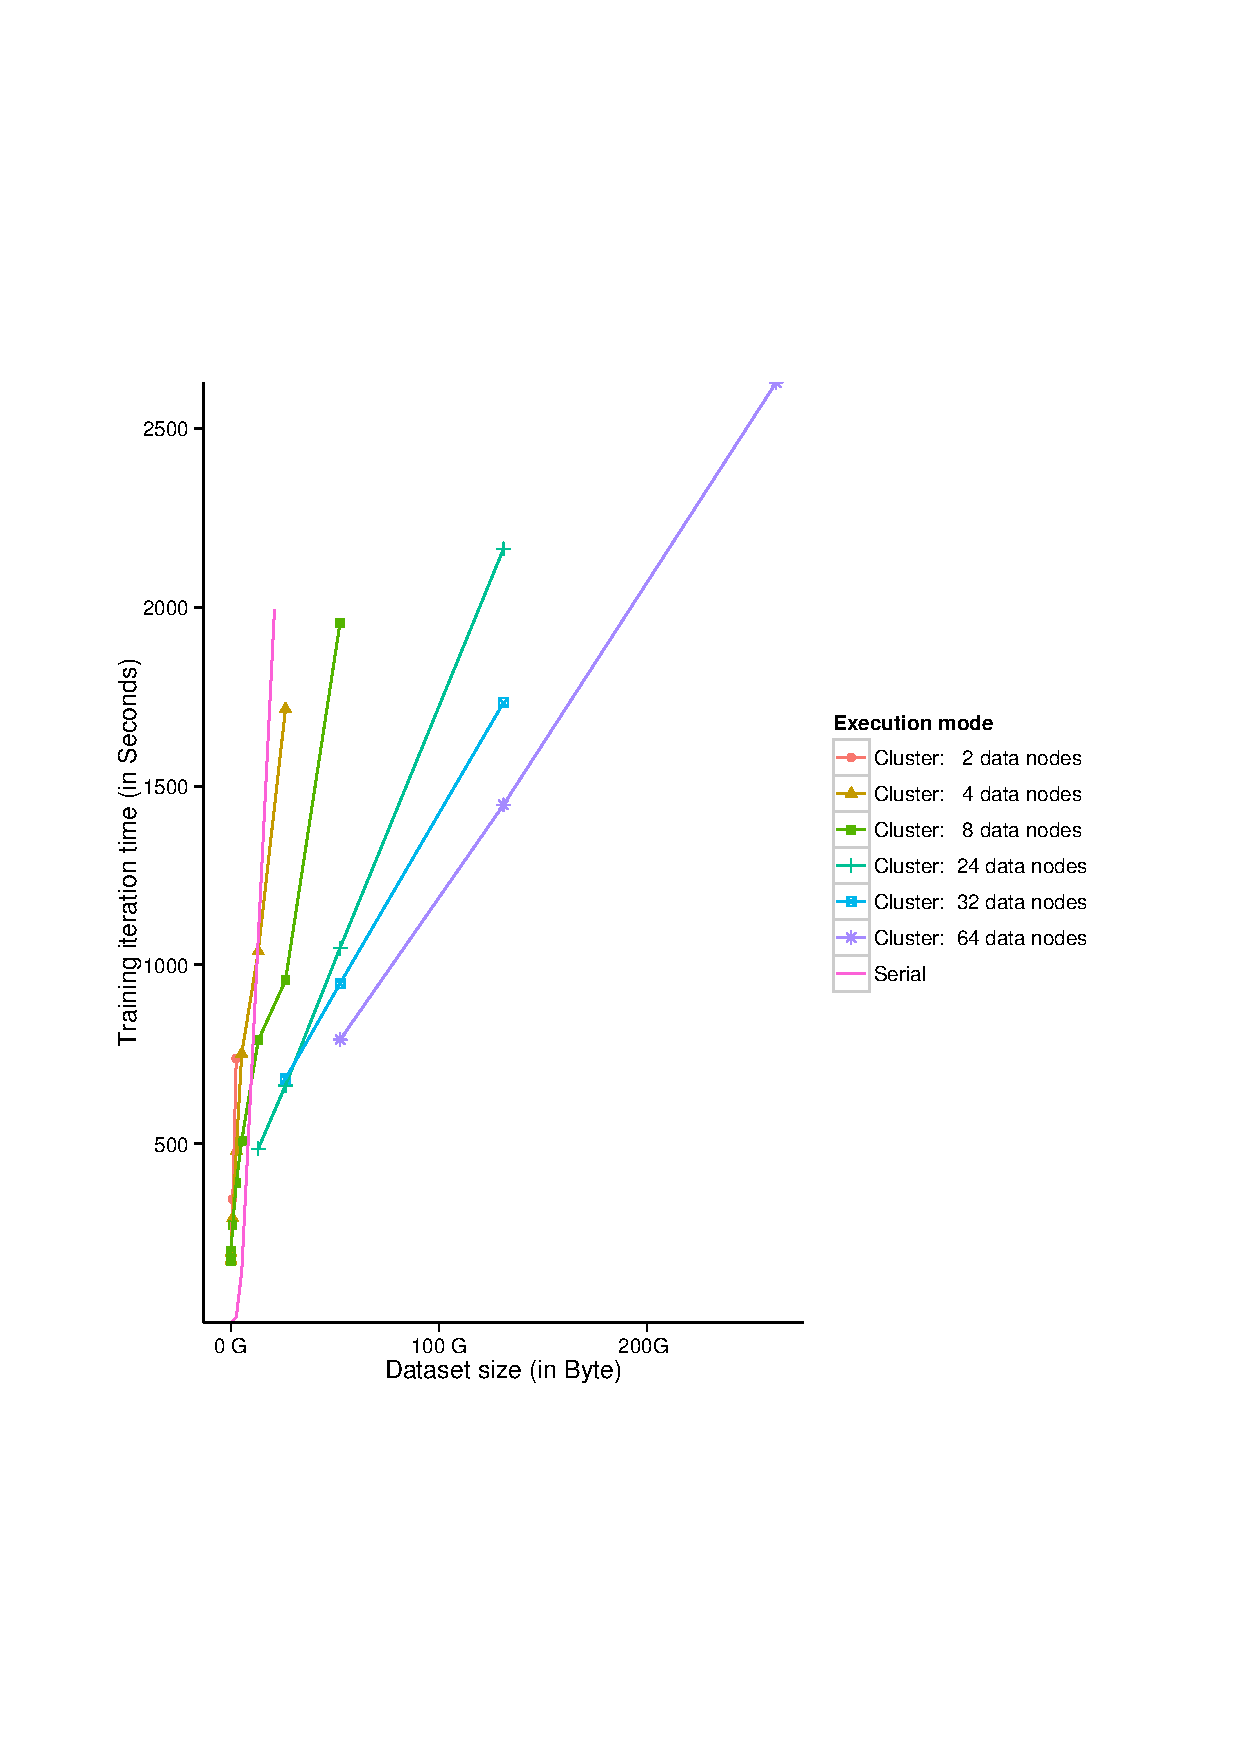
\includegraphics[trim=0cm 5cm 0cm 5cm, scale=0.7]{gfx/time_single.pdf}
\caption{Processing time of a single ListNet training iteration}
\label{fig:listnet_train_time}
\end{figure}

\begin{figure}
\centering
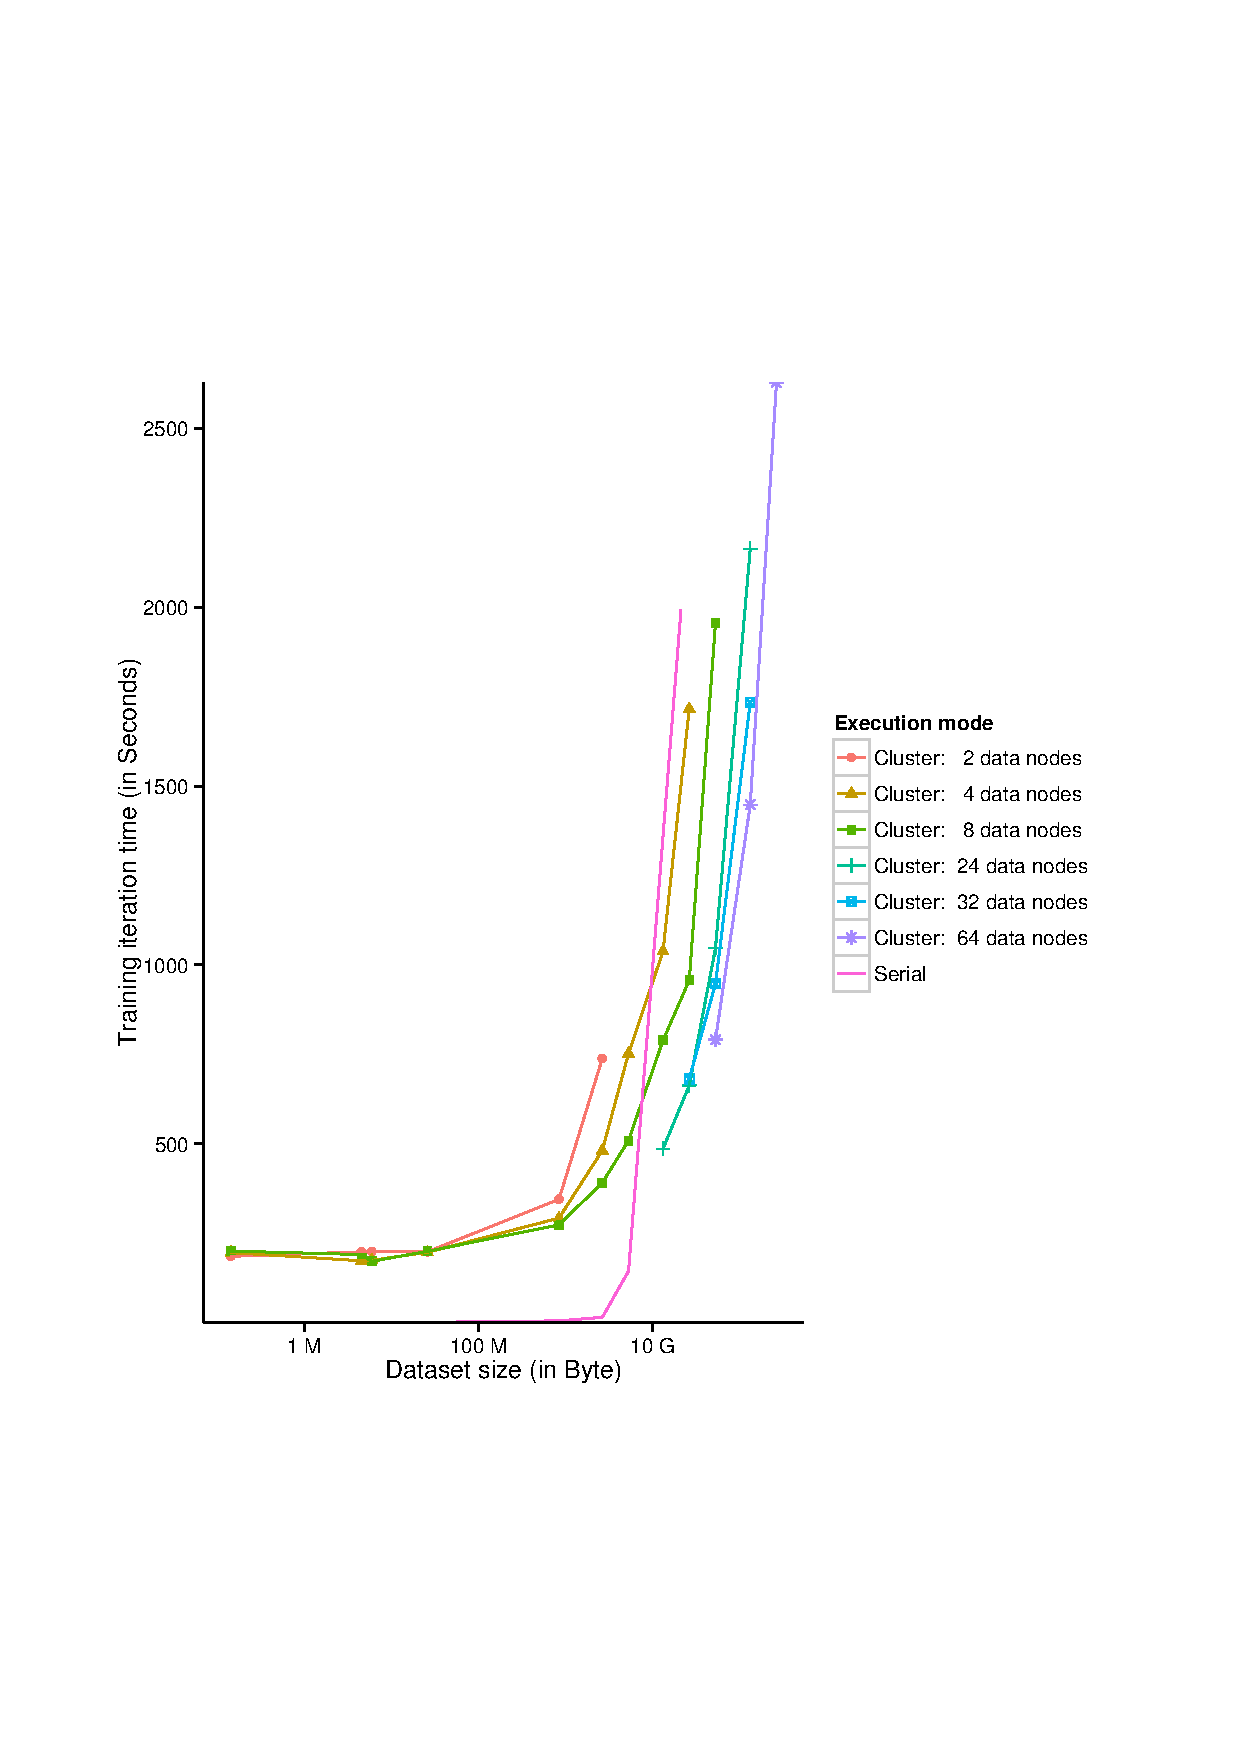
\includegraphics[trim=0cm 5cm 0cm 5cm, scale=0.7]{gfx/time_single_logx.pdf}
\caption{Processing time of a single ListNet training iteration on a logarithmic scale}
\label{fig:listnet_train_time_log}
\end{figure}

\begin{figure}
\centering
\includegraphics[trim=0cm 5cm 0cm 5cm, scale=0.7]{gfx/throughput_single_logx.pdf}
\caption{Throughput of a ListNet training iteration}
\label{fig:listnet_throughput}
\end{figure}
\part{Conclusions}
Using our experimental results we will now reflect on our research questions stated in the \ref{sec:goals} section of this thesis. We formulated the following research questions:
\begin{description}
\item[RQ1] What are the best performing Learning to Rank algorithms in terms of ranking accuracy on relevant benchmark data sets?
\end{description}
To answer this research question we proposed a new way of comparing learning to rank methods based on sparse evaluation results data on a set of benchmark datasets. Our comparison methodology comprises of two components: 1) \ac{NWN}, which provides insight in the ranking accuracy of the learning to rank method, and 2) \ac{IWN}, which gives insight in the degree of certainty concerning the performance of the ranking accuracy. Based on our literature search for evaluation results on well-known benchmarks collections, insight has been gained with the cross-benchmark comparison on which methods tend to perform better than others. However, no closing arguments can be formulated on which learning to rank methods are most accurate. LRUF, FSMRank, FenchelRank, SmoothRank and ListNet were the learning to rank algorithms for which it holds that no other algorithm produced more accurate rankings with a higher degree of certainty of ranking accuracy. From left to right, the ranking accuracy of these methods decreases while the certainty of the ranking accuracy increases. More evaluation runs are needed to increase the certainty of the ranking accuracy of the methods that were found to have low \ac{IWN} values. Our work contributes to this by identifying promising learning to rank methods that researchers could focus on in performing additional evaluation runs.

\begin{description}
\item[RQ2] What is the speed-up of those Learning to Rank algorithms when executed using the MapReduce framework?
\end{description}
\bigskip
Where the definition of \emph{relative speed-up} is used for speed-up \cite{Sun1991}:\\

$S_N = \frac{\text{execution time using one core}}{\text{execution time using \emph{N} cores}}$\\

To answer this research question, we took the approach of implementing the list of algorithms found in answering the first research question, starting with the Learning to Rank method with the highest certainty on ranking accuracy, ListNet.\\

We found that running ListNet on a Hadoop cluster using the MapReduce computing model comes with its own cost in the form of a job scheduling overhead in the range of 150-200 seconds per training iteration. This makes Hadoop very inefficient for the processing of small data sets, where the Hadoop overhead tends to make up a large share of the total processing time. For small data sets where the constant 150-200 seconds job scheduling overhead is a large fraction of the total processing time, single-machine computation, which does not have this job scheduling overhead, is found to be faster than Hadoop MapReduce computation. For large data sets, where 150-200 seconds overhead per iteration is small compared to the total time that it would take to process the data, Hadoop MapReduce can provide a speed-up to the training process. ListNet on a single machine does not scale well to data sizes larger than the physical memory size. To process large data sets with the ListNet training algorithm, Hadoop MapReduce is a large improvement compared to a single machine.\\

Moreover, we found that the addition of a normalisation preprocessing step to the ListNet procedure can greatly improve the ranking accuracy of the ListNet training procedure after the first five iterations. This suggests that the addition of a normalisation preprocessing step can reduce the number of training iterations needed for convergence. Lin stated in his essay \cite{Lin2013} that MapReduce is often good enough for tasks that are not-amenable to the MapReduce model. Lin motivates this statement in the context of iterative algorithms with the observation that these iterative algorithms can often be optimised in such a way that less iterations are needed for convergence. Our preprocessing step can improve the convergence rate of the ListNet training iteration, and therefore fits into Lin's point of view.\\

Most importantly, we found the training time of our cluster version of ListNet to grow better than linearly in terms of data size increase. This shows that the cluster implementation of ListNet can be used to scale the ListNet training procedure to arbitrarily large data sets, given that enough data nodes are available for computation.\\

No generalisations can be drawn from these results to the scalability on MapReduce of other Learning to Rank algorithms. However, we can extend our findings on job scheduling overhead and scaling benefit on large data sets to the gradient descent procedure that is used in ListNet as well as in many other Learning to Rank algorithms and in many learning algorithms in general. Other Learning to Rank algorithms using the gradient descent procedure might not scale well when the MapReduce computing model is used, but any bad scaling behaviour on MapReduce of Learning to Rank algorithms will not be caused by bad scaling of the gradient descent procedure.


% ********************************************************************
% Backmatter
%*******************************************************
\appendix
\cleardoublepage
\part{Appendix}
%********************************************************************
% Appendix
%*******************************************************
% If problems with the headers: get headings in appendix etc. right
%\markboth{\spacedlowsmallcaps{Appendix}}{\spacedlowsmallcaps{Appendix}}
\chapter{Appendix Test}
Lorem ipsum at nusquam appellantur his, ut eos erant homero
concludaturque. Albucius appellantur deterruisset id eam, vivendum
partiendo dissentiet ei ius. Vis melius facilisis ea, sea id convenire
referrentur, takimata adolescens ex duo. Ei harum argumentum per. Eam
vidit exerci appetere ad, ut vel zzril intellegam interpretaris.

Errem omnium ea per, pro congue populo ornatus cu, ex qui dicant
nemore melius. No pri diam iriure euismod. Graecis eleifend
appellantur quo id. Id corpora inimicus nam, facer nonummy ne pro,
kasd repudiandae ei mei. Mea menandri mediocrem dissentiet cu, ex
nominati imperdiet nec, sea odio duis vocent ei. Tempor everti
appareat cu ius, ridens audiam an qui, aliquid admodum conceptam ne
qui. Vis ea melius nostrum, mel alienum euripidis eu.

\section{Appendix Section Test}
Ei choro aeterno antiopam mea, labitur bonorum pri no. His no decore
nemore graecis. In eos meis nominavi, liber soluta vim cu. Sea commune
suavitate interpretaris eu, vix eu libris efficiantur.

\graffito{More dummy text.}
Nulla fastidii ea ius, exerci suscipit instructior te nam, in ullum
postulant quo. Congue quaestio philosophia his at, sea odio autem
vulputate ex. Cu usu mucius iisque voluptua. Sit maiorum propriae at,
ea cum primis intellegat. Hinc cotidieque reprehendunt eu nec. Autem
timeam deleniti usu id, in nec nibh altera.

\section{Another Appendix Section Test}
Equidem detraxit cu nam, vix eu delenit periculis. Eos ut vero
constituto, no vidit propriae complectitur sea. Diceret nonummy in
has, no qui eligendi recteque consetetur. Mel eu dictas suscipiantur,
et sed placerat oporteat. At ipsum electram mei, ad aeque atomorum
mea.

\begin{table}
    \myfloatalign
  \begin{tabularx}{\textwidth}{Xll} \toprule
    \tableheadline{labitur bonorum pri no} & \tableheadline{que vista}
    & \tableheadline{human} \\ \midrule
    fastidii ea ius & germano &  demonstratea \\
    suscipit instructior & titulo & personas \\
    %postulant quo & westeuropee & sanctificatec \\
    \midrule
    quaestio philosophia & facto & demonstrated \\
    %autem vulputate ex & parola & romanic \\
    %usu mucius iisque & studio & sanctificatef \\
    \bottomrule
  \end{tabularx}
  \caption[Autem usu id]{Autem usu id.}
  \label{tab:moreexample}
\end{table}

Ei solet nemore consectetuer nam. Ad eam porro impetus, te choro omnes
evertitur mel. Molestie conclusionemque vel at, no qui omittam
expetenda efficiendi. Eu quo nobis offendit, verterem scriptorem ne
vix.

  
\begin{lstlisting}[float,caption=A floating example]
for i:=maxint to 0 do
begin
{ do nothing }
end;
\end{lstlisting}
%********************************************************************
% Other Stuff in the Back
%*******************************************************
\cleardoublepage%********************************************************************
% Bibliography
%*******************************************************
% work-around to have small caps also here in the headline
\manualmark
\markboth{\spacedlowsmallcaps{\bibname}}{\spacedlowsmallcaps{\bibname}} % work-around to have small caps also
%\phantomsection 
\refstepcounter{dummy}
\addtocontents{toc}{\protect\vspace{\beforebibskip}} % to have the bib a bit from the rest in the toc
\addcontentsline{toc}{chapter}{\tocEntry{\bibname}}
\bibliographystyle{plainnat}
\label{app:bibliography} 
\bibliography{Bibliography}
\cleardoublepage\pagestyle{empty}

\hfill

\vfill


\pdfbookmark[0]{Colophon}{colophon}
\section*{Colophon}
This document was typeset using the typographical look-and-feel \texttt{classicthesis} developed by Andr\'e Miede. 
The style was inspired by Robert Bringhurst's seminal book on typography ``\emph{The Elements of Typographic Style}''. 
\texttt{classicthesis} is available for both \LaTeX\ and \mLyX: 
\begin{center}
\url{http://code.google.com/p/classicthesis/}
\end{center}
Happy users of \texttt{classicthesis} usually send a real postcard to the author, a collection of postcards received so far is featured here: 
\begin{center}
\url{http://postcards.miede.de/}
\end{center}
 
\bigskip

\noindent\finalVersionString

%Hermann Zapf's \emph{Palatino} and \emph{Euler} type faces (Type~1 PostScript fonts \emph{URW
%Palladio L} and \emph{FPL}) are used. The ``typewriter'' text is typeset in \emph{Bera Mono}, 
%originally developed by Bitstream, Inc. as ``Bitstream Vera''. (Type~1 PostScript fonts were made 
%available by Malte Rosenau and
%Ulrich Dirr.)

%\paragraph{note:} The custom size of the textblock was calculated
%using the directions given by Mr. Bringhurst (pages 26--29 and
%175/176). 10~pt Palatino needs  133.21~pt for the string
%``abcdefghijklmnopqrstuvwxyz''. This yields a good line length between
%24--26~pc (288--312~pt). Using a ``\emph{double square textblock}''
%with a 1:2 ratio this results in a textblock of 312:624~pt (which
%includes the headline in this design). A good alternative would be the
%``\emph{golden section textblock}'' with a ratio of 1:1.62, here
%312:505.44~pt. For comparison, \texttt{DIV9} of the \texttt{typearea}
%package results in a line length of 389~pt (32.4~pc), which is by far
%too long. However, this information will only be of interest for
%hardcore pseudo-typographers like me.%
%
%To make your own calculations, use the following commands and look up
%the corresponding lengths in the book:
%\begin{verbatim}
%    \settowidth{\abcd}{abcdefghijklmnopqrstuvwxyz}
%    \the\abcd\ % prints the value of the length
%\end{verbatim}
%Please see the file \texttt{classicthesis.sty} for some precalculated 
%values for Palatino and Minion.
%
%    \settowidth{\abcd}{abcdefghijklmnopqrstuvwxyz}
%    \the\abcd\ % prints the value of the length





\cleardoublepage%*******************************************************
% Declaration
%*******************************************************
\refstepcounter{dummy}
\pdfbookmark[0]{Declaration}{declaration}
\chapter*{Declaration}
\thispagestyle{empty}
Put your declaration here.
\bigskip
 
\noindent\textit{\myLocation, \myTime}

\smallskip

\begin{flushright}
    \begin{tabular}{m{5cm}}
        \\ \hline
        \centering\myName \\
    \end{tabular}
\end{flushright}

% ********************************************************************
% Game Over: Restore, Restart, or Quit?
%*******************************************************
\end{document}
% ********************************************************************
